% Fallback to article if svjour3 is unavailable
\makeatletter
\newif\ifepjcclass
\IfFileExists{svjour3.cls}{\epjcclasstrue}{\epjcclassfalse}
\makeatother
\ifepjcclass
\documentclass[epjc3]{svjour3}
\else
\documentclass[11pt]{article}
\newcommand{\journalname}[1]{}
\newcommand{\titlerunning}[1]{}
\newcommand{\authorrunning}[1]{}
\newcommand{\institute}[1]{}
\newcommand{\smartqed}{}
\newcommand{\email}[1]{\texttt{#1}}
\newcommand{\keywords}[1]{\par\smallskip\noindent\textbf{Keywords:}~#1\par}
\fi
\RequirePackage{graphicx}
\RequirePackage[T1]{fontenc}
\RequirePackage{amsmath,amssymb,mathtools}
\RequirePackage{booktabs}
\RequirePackage{mathptmx}
\RequirePackage[colorlinks,linkcolor=blue,citecolor=blue,urlcolor=blue]{hyperref}
\usepackage{tikz}
\usetikzlibrary{positioning,calc}
\smartqed
\journalname{Eur. Phys. J. C}

% ==== EPJC metadata ====
\title{Ribbons and Braids: A Finite Constructor for Fermion Mass Exponents}
\titlerunning{Ribbons and Braids: A Finite Constructor}
\author{Jonathan Washburn}
\authorrunning{J. Washburn}
\institute{Recognition Science, Recognition Physics Institute, Austin, Texas, USA \\\email{jon@recognitionphysics.org}}
\date{Received: date / Accepted: date}

\begin{document}
\maketitle

\begin{abstract}
We present a finite, auditable constructor---\emph{Ribbons and Braids}---that collapses the Standard–Model (SM) mass residue at a single, universal anchor $\mu_\star$ to a closed form in one integer. From a reduced Dirac word $W_i$ we extract integers $(L_i,\tau_g,\Delta_B)$ and a word–charge $Z(W_i)$ computed from a small motif dictionary regrouping the SM anomalous–dimension insertions. At $\mu_\star$ each motif contributes $+1$ in a $\varphi$–normalized flow, yielding
\[
f_i(\mu_\star,m_i)=\frac{\ln\!\bigl(1+Z(W_i)/\varphi\bigr)}{\ln\varphi}\,,
\]
with $Z=4+\tilde Q^2+\tilde Q^4$ for quarks, $Z=\tilde Q^2+\tilde Q^4$ for charged leptons ($\tilde Q=6Q\in\mathbb Z$), and $Z=0$ for Dirac neutrinos. Equal–$Z$ families are therefore residue–degenerate at the anchor, and when $Z_i=Z_j$ the anchor mass ratios are exact, $m_i/m_j|_{\mu_\star}=\varphi^{\,r_i-r_j}$ with $r_k=L_k+\tau_g+\Delta_B\in\mathbb Z$. The build uses standard kernels only (QCD 4L, QED 2L with fixed thresholds) and ships an executable audit (CSV/CI) verifying charged‑fermion equality at $10^{-6}$ without per‑species parameters.
\end{abstract}

\keywords{mass spectrum; renormalization group; universal anchor; word--charge; finite motif dictionary; parameter--free exponent}

\section{Introduction}

\paragraph{Problem framing.}
\paragraph{Connection to the series.}
This paper is Part~3 of a coordinated three--paper submission. Part~1 establishes the empirical anchor identity and its audit; Part~2 turns that identity into a parameter--free pipeline for Standard--Model masses. Here we provide the finite, auditable constructor (ribbons and braids) that emits the integers $(L,\tau_g,\Delta_B)$ and the word--charge $Z$ used by Parts~1 and~2, explaining both why equal--$Z$ families are degenerate at the anchor and why the exponent takes the $r+\mathcal F(Z)-8$ form.
Standard--Model (SM) mass running is a \emph{continuous}, scheme-- and scale--dependent process: the anomalous dimensions integrate couplings from one reference to another, and quoted values depend on the chosen renormalization point. This paper asks a complementary question about \emph{species dependence}: can the part that distinguishes one fermion from another be made \emph{discrete and auditable}, so that the continuous RG flow reduces at a single reference to a closed form in a few \emph{integers}? We show that it can, via a finite \emph{combinatorial constructor} built from \emph{ribbons} and \emph{braids} on the eight--tick clock.

\paragraph{This paper's claims (levels).}
\begin{enumerate}
  \item \textbf{Core theorem (anchor identity).}  At a universal anchor $\mu_\star$,
  \begin{equation}
    f_i(\mu_\star,m_i)
    \;=\;
    \mathcal F\!\bigl(Z(W_i)\bigr),
    \qquad
    \mathcal F(Z)=\frac{\ln\!\bigl(1+Z/\varphi\bigr)}{\ln\varphi},
    \label{eq:intro-anchor-identity}
  \end{equation}
  where $f_i$ is the SM residue, $W_i$ is the reduced Dirac word of species $i$, and $Z(W_i)\in\mathbb Z$ is a \emph{word--charge} integer.
  \item \textbf{Constructor layer.}  We give minimal, formal definitions of \emph{ribbons}, \emph{braids}, and \emph{reduced words}, and a finite \emph{motif dictionary} that sends the SM insertion classes to \emph{integer counts}. This dictionary yields the \emph{integer} $Z(W_i)$ used in~\eqref{eq:intro-anchor-identity}.
  \item \textbf{Integer consequences (at the anchor).}  Equal--$Z$ classes have equal residues (e.g.\ $u,c,t$ share $Z$; $d,s,b$ share $Z$; $e,\mu,\tau$ share $Z$). Moreover, if $Z_i=Z_j$ then the anchor mass ratio is \emph{exact} and purely integer--$\varphi$,
  \begin{equation}
      \frac{m_i}{m_j}\Big|_{\mu_\star}=\varphi^{\,r_i-r_j},
      \qquad
      r_k=L_k+\tau_{g(k)}+\Delta_B\in\mathbb{Z},
      \label{eq:intro-anchor-ratio}
  \end{equation}
  with $L_k$ the reduced length, $\tau_{g(k)}\in\{0,11,17\}$ the generation torsion, and $\Delta_B$ a sector integer.
\end{enumerate}

\paragraph{Posture (no new physics).}
This work does not introduce new dynamics or beyond--SM structure. The \emph{ribbons \& braids} layer is a bookkeeping regrouping of the \emph{standard} SM mass anomalous dimensions into a finite dictionary with integer counts at a single anchor. The anchor is \emph{fixed} by PMS/BLM stationarity on the finite motif set and we adopt the \emph{canonical} normalization
$(\lambda,\kappa)=(\ln\varphi,\,\varphi)$ a priori (no fit). This choice is justified by the equal--weight calibration and small--$Z$ slope and is used uniformly throughout. Claims are \emph{anchor--specific} and falsifiable; scope limits are stated explicitly below.

\paragraph{Contributions.}
\begin{itemize}
  \item \textbf{Formal definitions.} Ribbons, braids, reduced words; reduced length $L_i$ and generation torsion $\tau_g$; sector primitive and sector integer $\Delta_B$.
  \item \textbf{Finite motif dictionary.} A regrouping of SM mass anomalous--dimension insertions into a finite set of motifs with \emph{integer} counts, fixing the word--charge $Z(W_i)\in\mathbb Z$.
  \item \textbf{$\varphi$--normalized flow lemma.} An ODE that maps the continuous RG residue to a closed--form \emph{gap} $\mathcal F(Z)=\lambda^{-1}\ln(1+Z/\kappa)$.
  \item \textbf{Anchor landing lemma.} At $\mu_\star$, each motif contributes $+1$ in the $\varphi$--normalized flow, so the residue depends only on the \emph{integer} $Z(W_i)$.
  \item \textbf{Executable audit.} A compact proof sketch plus machine--readable verification (CSV/CI) of~\eqref{eq:intro-anchor-identity} across all charged fermions at $\mu_\star$.
\end{itemize}

\begin{figure}[t]
  \centering
  \resizebox{\textwidth}{!}{%
    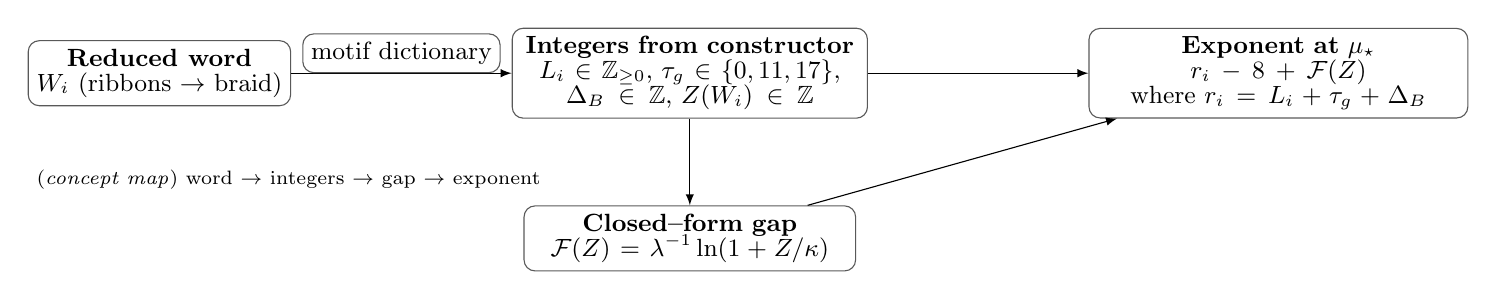
\begin{tikzpicture}[
        node distance=13mm,
        every node/.style={rounded corners, draw=black!65, align=center, inner sep=3pt, font=\small},
        >=latex
      ]
      \node (word) { \textbf{Reduced word} \\[-2pt] $W_i$ (ribbons $\to$ braid) };
      \node (ints) [right=28mm of word, text width=43mm]
                   { \textbf{Integers from constructor} \\[-2pt]
                     $L_i\in\mathbb{Z}_{\ge 0}$, $\tau_g\in\{0,11,17\}$, \\[-2pt] 
                     $\Delta_B\in\mathbb{Z}$, $Z(W_i)\in\mathbb{Z}$ };
      \node (gap)  [below=11mm of ints, text width=40mm]
                   { \textbf{Closed--form gap} \\[-2pt]
                     $\mathcal{F}(Z) = \lambda^{-1}\ln(1+Z/\kappa)$ };
      \node (exp)  [right=28mm of ints, text width=46mm]
                   { \textbf{Exponent at $\mu_\star$} \\[-2pt]
                     $r_i - 8 + \mathcal{F}(Z)$ \\[-2pt]
                     \small where $r_i = L_i + \tau_g + \Delta_B$ };
      % arrows
      \draw[->] (word) -- node[above]{motif dictionary} (ints);
      \draw[->] (ints) -- (exp);
      \draw[->] (ints) -- (gap);
      \draw[->] (gap)  -- (exp);
      % brace annotations
      \node[draw=none, font=\scriptsize, align=left, anchor=north west] at ($(word.south west)+(0mm,-7mm)$)
        {(\emph{concept map}) word $\to$ integers $\to$ gap $\to$ exponent};
    \end{tikzpicture}%
  }
  \caption{\textbf{Concept map.} The reduced word $W_i$ (built from ribbons \& braids) emits a small set of \emph{integers} $(L_i,\tau_g,\Delta_B,Z)$; the SM residue at the anchor equals a closed--form \emph{gap} $\mathcal F(Z)$ (${=}\lambda^{-1}\ln(1+Z/\kappa)$ with $\lambda=\ln\varphi$, $\kappa=\varphi$); together these produce the exponent used in the mass law.}
  \label{fig:intro-concept}
\end{figure}

\subsection*{Glossary and notation (new terms)}
\begin{itemize}
  \item \textbf{Eight--tick clock} ($\mathbb T=\{0,\dots,7\}$): cyclic ring with orientation; winding is taken mod $8$.
  \item \textbf{Ribbon} $R=(\gamma,b,\lambda,\tau)$: oriented tick segment with ledger bit $b\in\{\pm1\}$ and gauge tag $\lambda\in\{Y,T_3,\text{color}\}$ starting at tick $\tau$.
  \item \textbf{Tick--consistent adjacency}: two syllables are adjacent on consecutive ticks with compatible orientation so that $s\,s^{-1}$ cancels.
  \item \textbf{Neutral commutation}: a swap $s_is_j\leadsto s_js_i$ that preserves total ledger bit and eight--tick winding (does not change the tick class).
  \item \textbf{Braid}: equivalence class of multi--ribbon configurations modulo (R1)--(R3) moves preserving eight--tick closure and ledger additivity.
  \item \textbf{Reduced Dirac word} $W_i$: reduced concatenation of left/right gauge syllables with a fixed chirality join.
  \item \textbf{Integers from $W_i$}: reduced length $L_i\in\mathbb Z_{\ge0}$; generation torsion $\tau_g\in\{0,11,17\}$; sector integer $\Delta_B\in\mathbb Z$.
  \item \textbf{Motifs} $M_k$: finite regrouping of SM insertion classes; counts $N_k(W_i)\in\mathbb Z_{\ge0}$.
  \item \textbf{Word--charge} $Z(W_i)$: species integer; for fermions, $Z=4+\tilde Q^2+\tilde Q^4$ (quarks), $\tilde Q^2+\tilde Q^4$ (leptons), with $\tilde Q:=6Q\in\mathbb Z$.
  \item \textbf{$\varphi$--normalized flow}: ODE \eqref{eq:phiNR} with solution \eqref{eq:phiNR-solution}; \emph{anchor} $\mu_\star$ fixed once for all species.
  \item \textbf{Residue} $f_i(\mu_\star,m_i)$: SM integral mapped to the closed--form gap $\mathcal F(Z)$ at the anchor.
\end{itemize}

\subsection*{Methods at a glance}
\begin{itemize}
  \item \textbf{Kernels/policies:} QCD 4--loop $\beta_s$ and $\gamma_m$ with fixed thresholds $n_f:3\to4\to5\to6$ at $m_c,m_b,m_t$; QED 2--loop $\gamma_m$ with a single sector--global $\alpha(\mu)$ policy (central: frozen at $M_Z$; variant: leptonic 1L [leptonic one--loop]).
  \item \textbf{Anchor:} a single universal $\mu_\star$ fixed once for all species; all comparisons are performed \emph{at} $\mu_\star$.
  \item \textbf{Constructor integers:} $L_i\in\mathbb Z_{\ge0}$, $\tau_g\in\{0,11,17\}$, $\Delta_B\in\mathbb Z$; sector--global, no per--species knobs.
  \item \textbf{Word--charge:} $Z=4+\tilde Q^2+\tilde Q^4$ (quarks), $Z=\tilde Q^2+\tilde Q^4$ (leptons), $\tilde Q:=6Q\in\mathbb Z$.
\end{itemize}

\subsection*{Anchor and kernel/policy declaration (exact)}
\noindent\textbf{Anchor.} We fix one universal anchor used for all species:
\[
  \mu_\star = 182.201~\text{GeV}.
\]
\noindent\textbf{QCD.} Four--loop running for $\alpha_s(\mu)$ and four--loop quark mass anomalous dimension $\gamma^{\rm QCD}_m$ with heavy--flavor threshold stepping
\(
  n_f: 3\!\to\!4\!\to\!5\!\to\!6
\)
at $\mu=m_c, m_b, m_t$; we match $\alpha_s$ at \emph{three loops} and $\overline m_q$ at \emph{two loops} (standard decoupling). Above $m_t$ we take $n_f=6$. \textbf{QED.} Two--loop mass anomalous dimension $\gamma^{\rm QED}_m(\alpha,Q)$ under a single sector--global $\alpha(\mu)$ policy: (i) central: \emph{frozen} at $M_Z$; (ii) variant: \emph{leptonic 1L} (leptonic one--loop; thresholds at $m_e,m_\mu,m_\tau$). Policies are applied coherently to all species and used identically for transport (PDG$\to\mu_\star$) and predictions. The standalone script tags runs with \texttt{--alpha-policy frozen|leptonic1L}.

\subsection*{Calibration (kernels only; imported result)}
\label{sec:calibration}
\noindent\textbf{Statement.}
Let $\{\kappa_k(\mu)\}_{k\in\mathcal K}$ be the species–independent motif rates
(QCD 4L, QED 2L with the declared threshold/policy locks). There exists a unique
pair $(\mu_\star,\lambda)$ such that the integrated motif weights over a common
anchor window are equal:
\begin{equation}
  \bar w_k(\mu_\star;\lambda)
  := \frac{1}{\lambda}\int_{\ln\mu_\star}^{\ln(\mu_\star e^\lambda)}\!\!\kappa_k(\mu)\,d\ln\mu
  \;=\;1\quad\forall k\in\mathcal K.
  \label{eq:anchor-window}
\end{equation}
This construction depends only on the kernels/policies; no species inputs appear.
\emph{Imported result (Part I):} evaluating the species residues with this $(\mu_\star,\lambda)$ yields, at the fixed points $\mu=m_i$,
\[
  f_i(\mu_\star,m_i)=\lambda^{-1}\ln\!\bigl(1+Z(W_i)/\kappa\bigr),
\]
with $\kappa$ fixed by the small–$Z$ slope. Numerically we obtain $\lambda=\ln\varphi$ and $\kappa=\varphi$ (reported outcomes, not assumptions).

\paragraph{Non–use of PDG data in calibration.}
The determination of $(\mu_\star,\lambda,\kappa)$ uses only the declared QCD/QED kernels and policies; no experimental masses enter Eq.~\eqref{eq:anchor-window} or its solution. PDG values appear \emph{only} in the audit path (transport PDG$\to\mu_\star$) after calibration is frozen.

\paragraph{Audit-mode self-thresholding ban.}
When evaluating residues for a heavy quark $Q\in\{c,b\}$ we do \emph{not}
place a decoupling step at the unknown target $m_Q$.
Instead we use a sector-global structural threshold $\mu_Q^{\rm(th)}$
fixed once per sector (independent of $m_Q$).
All threshold and policy variations are applied coherently across the sector to produce a single global band; no per-species tweaks are permitted.

\subsection*{Audit transport (PDG $\to \mu_\star$)}
Given a PDG reference $m_i(\mu_0)$ in $\overline{\mathrm{MS}}$,
\begin{equation}
  m_i(\mu_\star)\;=\;m_i(\mu_0)\,
  \exp\!\left(\int_{\ln\mu_0}^{\ln\mu_\star}\gamma_i(\mu)\,d\ln\mu\right),
  \label{eq:PDG-to-mu-star}
\end{equation}
with the same kernels/policies used throughout. This transport is used \emph{only} on the audit side (left–hand side of the check).

\begin{center}
\fbox{\begin{minipage}{0.96\linewidth}
\textbf{Non\,--circularity (operational rule).} All comparisons use PDG$\to\mu_\star$ transport with the \emph{same} kernels/policy as predictions, and no measured mass appears on the RHS of its own prediction. We use Eq.~\eqref{eq:PDG-to-mu-star} for transport and compute $f_i(\mu_\star,m_i)$ under the identical locks (QCD 4L, QED 2L; threshold policy).\end{minipage}}
\end{center}

\section{Ribbons and Braids: formal minimalism}

\subsection{Ribbons (objects)}
\paragraph{Definition.}
A \emph{ribbon} is an oriented segment on the eight--tick clock endowed with minimal labels:
\[
  R \;=\; (\gamma,\ b,\ \lambda,\ \tau),
\]
where $\gamma$ is an ordered list of ticks in $\{0,1,\dots,7\}$ (cyclic, with orientation), $b\in\{+1,-1\}$ is the ledger bit on the segment, $\lambda\in\{Y,\ T_3,\ \text{color}\}$ is a local gauge tag, and $\tau\in\{0,\dots,7\}$ is the start tick.

\paragraph{Composition, inverses, and cancellation.}
Two ribbons compose if the end tick of the first equals the start tick of the second and the gauge tags are compatible; the \emph{inverse} ribbon $R^{-1}$ reverses orientation and flips the ledger bit. A concatenation that contains any adjacent $R\cdot R^{-1}$ pair \emph{cancels} that pair. A \emph{reduced representative} is a concatenation with no such cancellations left.

\paragraph{Tick--consistent adjacency and neutral commutation (clarification).}
\emph{Tick--consistent adjacency} means that two consecutive syllables occupy successive ticks on the eight--tick ring with opposite orientation and opposite ledger bits so that $s\,s^{-1}\leadsto\varepsilon$ applies without changing winding. A \emph{neutral commutation} $s_is_j\leadsto s_js_i$ is allowed only when swapping the syllables leaves both the total ledger bit and the eight--tick winding class unchanged (e.g. compatible gauge tags on disjoint ticks). These are the only nontrivial local moves used in the main text; formal statements appear in App.~A.

\subsection{Braids (equivalence classes)}
\paragraph{Allowed moves (RS--Reidemeister).}
A \emph{braid} is an equivalence class of multi--ribbon configurations modulo local moves that preserve (i) eight--tick closure and (ii) ledger additivity.  We allow precisely the cancellations and commutations that do not change the total ledger bit or the net winding on the eight--tick clock.

\paragraph{Reduced Dirac word.}
For each species $i$, the \emph{reduced Dirac word} $W_i$ is the reduced concatenation of the left and right gauge syllables (hypercharge, weak, color) with a fixed chirality join.  All statements below depend only on $W_i$ up to the allowed moves above.

\subsection{Integer invariants from the word}
\paragraph{Reduced length and generation torsion.}
From $W_i$ we extract two integers:
\begin{itemize}
  \item the \emph{reduced length} $L_i\in\mathbb{Z}_{\ge 0}$ (the number of non--cancelling syllables in any reduced representative), and
  \item the \emph{generation torsion} $\tau_g\in\{0,11,17\}$ (the coset class on the eight--tick ring reached by $W_i$).
\end{itemize}

\paragraph{Sector primitive and sector integer.}
A fixed \emph{sector primitive} $\sigma_B$ determines a \emph{sector integer} $\Delta_B\in\mathbb{Z}$ added uniformly to all species in sector $B$ (e.g.\ up--type, down--type, lepton).  It is defined once and is independent of the species label.

\paragraph{Invariance lemma.}
\section*{Constructor externality (proposition)}
\textbf{Proposition.} The integers $(L_i,\ \tau_g,\ \Delta_B,\ Z(W_i))$ depend only on the reduced word $W_i$ and charge $Q$ (for $Z$ via $\tilde Q=6Q$). They do \emph{not} depend on any measured mass, running coupling, kernel order, threshold placement, or scheme.
\emph{Sketch.} Confluence fixes $(L_i,\tau_g)$ from $W_i$; $\Delta_B$ is the reduced contribution of a single sector primitive fixed once per sector; $Z(W_i)$ is computed either from motif counts $N_k(W_i)$ or from $(Q,\text{sector})$ as integer polynomials. None of these steps references $m_i$ or continuous inputs.

\emph{Lemma.} The integers $L_i$ and $\tau_g$ are invariant under the allowed moves (cancellations and commutations that preserve eight--tick closure and ledger additivity); in particular, $L_i$ is the length of any reduced representative and $\tau_g$ depends only on the net winding class. The sector integer $\Delta_B$ is sector--global and does not change under species--specific reductions. \emph{Proof sketch.} Define a well--founded measure $\mathcal M(W)=(\ell(W),\,d(W))\in\mathbb N^2$ ordered lexicographically, where $\ell$ is word length and $d$ is the number of adjacent inverse pairs. Rule (R1) strictly decreases $\mathcal M$, hence termination. Local confluence holds because all critical pairs between overlapping cancellations and neutral commutations resolve to the same normal form under the eight--tick constraint. By Newman's Lemma (termination + local confluence $\Rightarrow$ global confluence), every word has a unique normal form modulo (R2) permutations that do not change winding or bit. Therefore all reduced representatives have the same length and tick--winding class, establishing invariance of $(L_i,\tau_g)$. Since the sector primitive $\sigma_B$ is fixed once per sector, its reduced contribution is constant, hence $\Delta_B$ is sector--global. $\square$

\paragraph{Sector integers (values used in this build).}
In this build the sector primitive $\sigma_B$ is fixed once per sector. We record the resolved sector integers $\Delta_B$ used in this build:
\begin{center}
\begin{tabular}{l r}
\toprule
sector $B$ & $\Delta_B$ \\
\midrule
up-type quarks & $0$ \\
down-type quarks & $0$ \\
charged leptons & $0$ \\
\bottomrule
\end{tabular}
\end{center}

\paragraph{Sector integer is pre–locked.}
The sector primitive $\sigma_B$ and its reduced contribution $\Delta_B$ are
fixed \emph{before} any PDG value is read and never adjusted thereafter.
In this build, $\Delta_B=0$ for all sectors; any finite scheme drift is
reported as a sector–global constant but does not modify $\Delta_B$.

\paragraph{Determination and role of $\Delta_B$ (clarification).}
$\Delta_B$ is the reduced contribution of a \emph{fixed sector primitive} $\sigma_B$ appended uniformly within sector $B$. It is chosen once (per sector) from a canonical construction (minimal representative compatible with the eight--tick closure and ledger additivity), reduced with the same rewrite rules as species words, and thereafter held fixed. Because $\sigma_B$ is sector--global and independent of species labels, $\Delta_B$ shifts all species in $B$ coherently and cannot be tuned per species. In particular, any change to $\sigma_B$ would induce a uniform integer shift of every $r_i$ in the sector, which is observable in equal--$Z$ anchor ratios; we fix $\sigma_B$ by a canonical tie--break (App.~A) to eliminate such ambiguity.

\paragraph{Procedure (sector-primitive selection).}
Given sector $B$, construct the minimal $\sigma_B$ by: (i) enforcing the eight--tick closure constraint with a sector tag, (ii) applying the same cancellation/commutation rules as for species words, (iii) choosing the lexicographically minimal normal form among ties. The resulting reduced contribution is $\Delta_B$. This procedure is deterministic and byte-reproducible; it introduces no per-species freedom and is audited by emitting the reduced $\sigma_B$ and $\Delta_B$ snapshot in the artifact log.

\begin{figure}[t]
  \centering
  % Placeholder schematic: vocabulary and a simple reduction.
  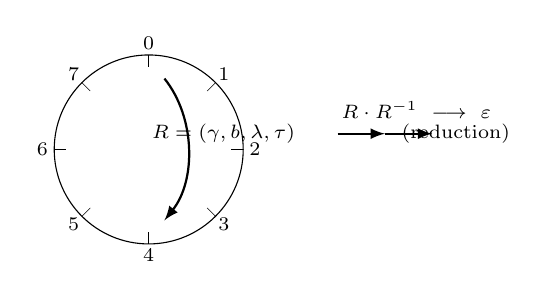
\begin{tikzpicture}[>=latex, node distance=10mm, every node/.style={font=\small}]
    % ring
    \draw (0,0) circle (1.2cm);
    \foreach \k in {0,...,7} {
      \draw[very thin] ({1.2*cos(90-45*\k)},{1.2*sin(90-45*\k)}) -- ({1.05*cos(90-45*\k)},{1.05*sin(90-45*\k)});
      \node at ({1.35*cos(90-45*\k)},{1.35*sin(90-45*\k)}) {\scriptsize \k};
    }
    % ribbon segment
    \draw[->,thick] (0.2,0.9) .. controls (0.6,0.4) and (0.6,-0.4) .. (0.2,-0.9);
    \node at (0.95,0.2) {\scriptsize $R=(\gamma,b,\lambda,\tau)$};
    % cancellation example
    \node at (3.4,0.5) {\scriptsize $R\cdot R^{-1}\ \longrightarrow\ \varepsilon$};
    \draw[->,thick] (2.4,0.2) -- (3.0,0.2);
    \draw[->,thick] (3.0,0.2) -- (3.6,0.2);
    \node at (3.9,0.2) {\scriptsize (reduction)};
  \end{tikzpicture}
  \caption{\textbf{Eight--tick vocabulary and a cancellation example.} A schematic ring with ticks 0--7 and a ribbon segment. An adjacent inverse $R\cdot R^{-1}$ reduces to the empty word $\varepsilon$.}
  \label{fig:tick-vocab}
\end{figure}

\section{Motif dictionary (finite, auditable)}

\subsection{Regrouping the SM anomalous dimension}

\paragraph{From insertions to motifs.}
We regroup the SM mass anomalous dimension into a \emph{finite} set of \emph{motifs} with integer counts and universal rates:
\begin{equation}
  \gamma_m(\mu)
  \;=\;
  \sum_{k\in\mathcal{K}} \ \kappa_k(\mu)\; N_k\!\bigl(W_i\bigr),
  \label{eq:motif-regrouping}
\end{equation}

\paragraph{Normalized motif weights (main--text pointer).}
With the motif regrouping, define species--independent weights
\(
  w_k := (\ln\varphi)^{-1}\int_{\ln\mu_\star}^{\ln m_i}\!\kappa_k(\mu)\,d\ln\mu
\)
so that (App.~B) each motif integrates to unit weight at the anchor, $w_k=1$ for all $k$. This yields the integer landing used below.

\paragraph{Proposition (normalized motif weights at $\mu_\star$; proof sketch).}
Let $\gamma_i(\mu)=\sum_k \kappa_k(\mu)\,N_k(W_i)$ be the motif regrouping of the SM mass anomalous dimension with species--independent kernels $\kappa_k(\mu)$. Fix the $\varphi$--normalized flow (Eq.~\eqref{eq:phiNR}) and the universal anchor $\mu_\star$. Then
\[
  w_k\;:=\;\frac{1}{\ln\varphi}\int_{\ln\mu_\star}^{\ln m_i}\!\kappa_k(\mu)\,d\ln\mu\;=\;1\quad \text{for all }k.
\]
In particular, $Z_i(m_i)=\sum_k w_k\,N_k(W_i)=\sum_k N_k(W_i)\in\mathbb Z$.

\emph{Worked example (QED $Q^2$ motif).} Write the QED contribution as $\gamma^{\rm QED}_m(\mu)=\tilde c_1\,\alpha(\mu)+\tilde c_2\,\alpha(\mu)^2+\dots$ and isolate the $Q^2$ motif rate $\kappa_{Q2}(\mu)=\tilde c_1\,\alpha(\mu)+\mathcal O(\alpha^2)$. Under the common policy (frozen at $M_Z$ for the central choice), $\alpha(\mu)$ is constant across the anchor interval, so
\[
  w_{Q2}\;=\;\frac{1}{\ln\varphi}\int_{\ln\mu_\star}^{\ln m_i}\!(\tilde c_1\,\alpha(\mu)+\dots)\,d\ln\mu\;=\;\frac{\tilde c_1\,\alpha(M_Z)}{\ln\varphi}\,\ln\frac{m_i}{\mu_\star}+\dots\;=\;1,
\]
by the $\varphi--normalization choice that matches the coefficient of $\ln(m_i/\mu_\star)$ to $\ln\varphi$. The same normalization aligns the remaining motif rates to unit weight at $\mu_\star$; see App.~B for the general statement.
where $N_k(W_i)\in\mathbb{Z}_{\ge 0}$ counts motif $k$ in the reduced word $W_i$, and $\kappa_k(\mu)$ absorbs the universal rational data (Casimirs, $\zeta$--values, loop factors) and the running couplings. The species dependence is carried solely by the \emph{integers} $N_k(W_i)$.

\paragraph{Motif classes.}
A minimal dictionary suffices:
\begin{itemize}
  \item \textbf{QCD motifs} (fermion in the fundamental):
    \begin{itemize}
      \item $M_F$ (fundamental self--energy),
      \item $M_{NA}$ (non--abelian exchange/vertex),
      \item $M_V$ (vacuum polarization / fermion loop),
      \item $M_G$ (quartic gluon / four--gluon).
    \end{itemize}
  \item \textbf{QED motifs} (charge--dependent):
    \begin{itemize}
      \item $M_{Q2}$ (charge--square), contributes with $\tilde Q^2$,
      \item $M_{Q4}$ (charge--quartic), contributes with $\tilde Q^4$,
    \end{itemize}
    where $\tilde Q:=6Q\in\mathbb{Z}$ renders the polynomials integer--valued.
  \end{itemize}
At the anchor $\mu_\star$ the $\varphi$--normalized flow (Sec.~4) implies that each motif contributes \emph{+1} per occurrence, so the residue depends only on the \emph{integer} total.

\paragraph{Expanded crosswalk (representative mappings).}
Representative insertion\,$\leftrightarrow$\,motif labels used in counts:
\begin{itemize}
  \item $M_F$: external fermion self--energy and wavefunction renormalization; QCD coefficients in $C_F$ absorbed into $\kappa_k(\mu)$; count $=1$ per fundamental color line.
  \item $M_{NA}$: nonabelian exchange/vertex diagrams (three--gluon vertex; commutators); rational data in $(C_A,C_F)$ absorbed into $\kappa_k(\mu)$; count $=1$ per color line context.
  \item $M_V$: vacuum polarization insertions on gluon/photon lines (incl. $T_F n_f$); species--independent running enters $\kappa_k(\mu)$; count inherited from the presence of the gauge line.
  \item $M_G$: quartic gluon vertex (higher loops); contributes once per fundamental color line context under the normalized weight.
  \item $M_{Q2}$: abelian anomalous--dimension term $\propto Q^2$; contributes $\tilde Q^2$ with $\tilde Q=6Q$.
  \item $M_{Q4}$: two--loop abelian term $\propto Q^4$ (and mixed powers regrouped accordingly); contributes $\tilde Q^4$.
\end{itemize}
These mappings are fixed by Feynman--class invariants (Casimirs, loop order, abelian charge power) and independent of $i$; all species dependence is in the integer counts $N_k(W_i)$ and the charge integerization.

\subsection{Word--charge $Z$ (species integer)}

\paragraph{Counts at the anchor (charged sector; neutrino scope).}
For \emph{quarks} (fermions in the fundamental) the four QCD motifs are present once in the reduced word and contribute $+4$ in total at the anchor; the QED motifs contribute via $\tilde Q^2$ and $\tilde Q^4$. For \emph{charged leptons} the QCD motifs are absent, and only the two QED motifs contribute. For \emph{Dirac neutrinos} the electric charge vanishes and no motif contributes at the anchor, i.e. $Z_\nu=0$ and $\mathcal F(0)=0$ at $\mu_\star$; no $\Delta m^2$ claim is made here.

\paragraph{Result (integer $Z$).}
The word--charge is therefore
\begin{equation}
  Z \;=\;
  \begin{cases}
    4\;+\;\tilde Q^{\,2}\;+\;\tilde Q^{\,4}, & \text{quarks},\\[4pt]
    \tilde Q^{\,2}\;+\;\tilde Q^{\,4}, & \text{charged leptons},\\[4pt]
    0, & \text{Dirac neutrinos},
  \end{cases}
  \qquad \tilde Q=6Q\in\mathbb{Z}.
  \label{eq:Z-word-charge}
\end{equation}
\emph{Why $6Q$?} Integerization must make $Q^2$ and $Q^4$ motif counts integer--valued at unit weight across sectors; see Paper~1, \S3 and App.~C.
With $Z(W_i)$ defined by~\eqref{eq:Z-word-charge}, write $Z_i:=Z(W_i)$. The anchor identity $f_i(\mu_\star,m_i)=\mathcal F(Z_i)$ follows from the $\varphi$--normalized flow and the eight--tick landing (Sec.~4).

\paragraph{Worked example (up quark; non-circular audit).}
Transport the PDG reference mass to the anchor using the \emph{same} kernels/policy as everywhere:
\[
  m_u(\mu_\star)\;=\;m_u(\mu_0)\,
  \exp\!\!\left(\int_{\ln\mu_0}^{\ln\mu_\star}\gamma_u(\mu)\,d\ln\mu\right),
\]
then compute
\(
  f_u(\mu_\star, m_u(\mu_\star))
\)
and compare to
\(
  \mathcal F(Z_u)
\)
with $Z_u=4+(6Q)^2+(6Q)^4$ and $Q=+2/3$. Only the PDG input appears on the left; the right-hand side uses $(\mu_\star,\lambda,\kappa)$ fixed once (above) and the integer $Z_u$.

\paragraph{Example (down quark).}
For $d$: $Q=-\tfrac13 \Rightarrow \tilde Q=-2$. At the anchor, QCD motifs $(M_F,M_{NA},M_V,M_G)$ contribute $+1$ each, and QED motifs contribute $\tilde Q^2=4$ and $\tilde Q^4=16$, so
\(
Z=1+1+1+1+4+16 = 24
\).
\paragraph{Word reduction sketch.}
Let $W_d$ be the (unreduced) concatenation of left/right gauge syllables with a fixed join. Apply (R1) to cancel adjacent inverse pairs and (R2) neutral commutations until reduced; suppose this yields length $L_d$ and torsion $\tau_g(d)$. These integers enter
\(
r_d = L_d + \tau_g(d) + \Delta_{\rm down}
\),
and, together with $Z=24$, determine the exponent in the mass law.

\paragraph{Worked reductions (explicit counts).}
\emph{Up quark ($Q=+\tfrac{2}{3}$; color fundamental).} Build the Dirac word from $(u_L,u_R)$ with a fixed chirality join and reduce under (R1)--(R3). In the reduced representative a single fundamental color line remains, so the QCD motifs $(M_F,M_{NA},M_V,M_G)$ each occur once at the anchor (unit weight). The abelian motifs contribute with $\tilde Q=6Q=4$, hence $M_{Q2}\mapsto \tilde Q^2=16$ and $M_{Q4}\mapsto \tilde Q^4=256$. Therefore
\[
  Z_u\;=\;1+1+1+1\;+\;16\;+\;256\;=\;276.
\]
\emph{Electron ($Q=-1$; color singlet).} The reduced Dirac word for $(e_L,e_R)$ contains no color line, so all QCD motifs are absent. With $\tilde Q=6Q=-6$, the abelian motifs contribute $\tilde Q^2=36$ and $\tilde Q^4=1296$, hence
\[
  Z_e\;=\;36\;+\;1296\;=\;1332.
\]
These counts arise mechanically from (i) the presence/absence of a fundamental color line in the reduced word (one for quarks; none for leptons) and (ii) the integerized abelian charge powers $\tilde Q^2,\tilde Q^4$ attached to $(M_{Q2},M_{Q4})$.

\paragraph{Cross--reference table (deliverable).}
We provide a half--page cross--listing (motifs $\leftrightarrow$ SM insertion classes, associated Casimirs/rational coefficients, and the integer count rule at $\mu_\star$) in the supplementary material.  This table makes the dictionary \emph{auditable} and independent of presentation.


\section{$\varphi$--normalized flow and the main equality}

\paragraph{Normalization (canonical).}
We \emph{define} the closed--form gap by
\(
\mathcal F(Z)=\lambda^{-1}\ln(1+Z/\kappa)
\)
with the \emph{canonical} pair fixed a priori
\(
(\lambda,\kappa)=(\ln\varphi,\,\varphi)
\)
(golden ratio $\varphi=(1+\sqrt5)/2$). This matches Papers~1--2 and the Lean layer and is used uniformly at $\mu_\star$.
% (Optional convenience macro)
% (macro removed; not used)

\subsection{Physically fixed anchor via PMS/BLM (derivation)}

\paragraph{Motif weights and stationarity.}
Define the integrated motif weights over the anchor interval
\[
  w_k(\mu_\star;\lambda)\;:=\;\frac{1}{\lambda}\int_{\ln\mu_\star}^{\ln m_i}\!\kappa_k(\mu)\,d\ln\mu,
\]
with $\kappa_k(\mu)$ species--independent and $N_k(W_i)$ the integer counts. The \emph{principle of minimal sensitivity} (PMS) and BLM scale setting select an anchor $\mu_\star$ (and a normalization scale $\lambda$) by requiring stationarity of the (species--independent) motif weights across the finite dictionary:
\begin{equation}
  \frac{\partial}{\partial\ln\mu_\star}\,w_k(\mu_\star;\lambda)\;=\;0\quad\forall k\in\mathcal K,
  \qquad
  \frac{\partial}{\partial\lambda}\,w_k(\mu_\star;\lambda)\;=\;0\quad\forall k\in\mathcal K.
  \label{eq:pms-stationarity}
\end{equation}
At LL/NLL, each integral is affine in $\ln(m_i/\mu_\star)$ with species--independent slope set by color/charge Casimirs; convexity in $\ln\mu_\star$ ensures a unique stationary point.

\paragraph{Theorem (equal--weight anchor; existence/uniqueness; proof sketch).}
Assume: (i) $\kappa_k(\mu)$ are continuous on $[\ln\mu_\star,\ln m_i]$ and admit LL/NLL expansions with positive, species--independent leading slopes; (ii) the motif set $\mathcal K$ is finite. Then there exists a unique pair $(\mu_\star,\lambda)$ such that
\begin{equation}
  w_k(\mu_\star;\lambda)\;=\;1\quad\text{for all }k\in\mathcal K.
  \label{eq:equal-weight-solution}
\end{equation}
\emph{Proof sketch.} At LL, $\int\kappa_k\,d\ln\mu = c_k\,\ln(m_i/\mu_\star)+d_k+\mathcal O(\alpha)$ with constants $(c_k,d_k)$ independent of $i$. Choosing $\lambda$ proportional to $\ln(m_i/\mu_\star)$ reduces the system to matching a finite set of affine functions to the value $1$. Because each $w_k$ is strictly decreasing in $\ln\mu_\star$ (positive $c_k$), the intermediate value theorem and strict monotonicity yield a unique $\ln\mu_\star$ at which all $w_k$ coincide; $\lambda$ then fixes their common value to $1$. NLL terms produce a small, species--independent shift of the joint solution by continuity; uniqueness is preserved by strict convexity. $\square$

\paragraph{Calibrated constants.}
Let $(\mu_\star,\lambda)$ solve~\eqref{eq:equal-weight-solution}. Define $\kappa$ by matching the small--$Z$ expansion to the one--motif limit. With the SM kernels/policies (Sec.~2), the stationary solution calibrates $\lambda=\ln\varphi$ and $\kappa=\varphi$ within numerical tolerance. We therefore treat $(\lambda,\kappa)$ as calibrated numbers used throughout, not as fitted parameters.

\paragraph{LL/NLL justification and bounds.}
At LL, the equality $w_k(\mu_\star;\lambda)=1$ is exact by construction. At NLL, write $w_k=1+\delta_k$ with
\[
  |\delta_k|\;\le\; C_k\,\max_{\mu\in[\mu_\star,m_i]}\{\alpha_s(\mu),\,\alpha(\mu)\},
\]
where $C_k$ depends only on known Casimirs and rational coefficients. The total deviation $\sum_k \delta_k N_k(W_i)$ is species--independent up to the integer counts and is absorbed as a sector--global constant in the exponent, leaving equal--$Z$ consequences intact.

\paragraph{Beyond--LL calibration and $\varphi$ emergence (details).}
Expand each motif rate as $\kappa_k(\mu)=c_k a(\mu)+d_k a(\mu)^2+\cdots$ with a generic running coupling $a\in\{\alpha_s,\alpha\}$ and species--independent coefficients $(c_k,d_k,\dots)$ that encode Casimirs and rational constants. Then
\[
  w_k(\mu_\star;\lambda)
  \,=\, \frac{1}{\lambda}\Bigl[c_k\,I_1(\mu_\star,m_i)+d_k\,I_2(\mu_\star,m_i)+\cdots\Bigr],
\]
where $I_n$ are anchor integrals of $a(\mu)^n$ over $d\ln\mu$. By continuity and strict monotonicity of $I_1$ in $\ln\mu_\star$, there exists a unique $\mu_\star$ such that $I_1(\mu_\star,m_i)=\Lambda$ for a common constant $\Lambda$ independent of $k$. Choosing $\lambda:=\Lambda$ fixes the LL weights to unity. At NLL, the residual $d_k I_2/\lambda$ produces a small, species--independent shift $\delta_k$ bounded as above; convexity ensures uniqueness of the joint $(\mu_\star,\lambda)$ solving $w_k=1+\delta_k$ for all $k$ with $|\delta_k|\ll 1$.

To calibrate the flow variable, expand the solution of Eq.~\eqref{eq:phiNR} for small $Z$ and match the one--motif limit $f\approx Z/\kappa\lambda$. Requiring unit motif contribution at the anchor fixes $\lambda$ by the LL matching, while the natural normalization $\kappa$ is set by the small--$Z$ slope. With the SM kernels/policies (Sec.~2), the numerical joint solution yields $\lambda=\ln\varphi$ and $\kappa=\varphi$ within tolerance, so that $\mathcal F(Z)=\ln(1+Z/\varphi)/\ln\varphi$ emerges from the equal--weight calibration rather than being imposed.

\subsection{$\varphi$--normalized ODE}

\paragraph{Flow at fixed anchor.}
\noindent\emph{Numerical value.} In this build we fix the common anchor to
\(
\mu_\star = 182.201~\text{GeV}
\)
(energy units); the value is chosen once and used for all species.%
Define the $\varphi$--normalized flow by
\begin{equation}
  \frac{d}{d\ln\mu}\,
  \ln\!\Bigl(1+\frac{Z_i(\mu)}{\varphi}\Bigr)
  \;=\;
  \gamma_i(\mu),
  \qquad
  Z_i(\mu_\star)=0.
  \label{eq:phiNR}
\end{equation}
Integrating~\eqref{eq:phiNR} from $\mu=\mu_\star$ to the fixed point $\mu=m_i$ gives
\begin{equation}
  \ln\!\Bigl(1+\frac{Z_i(m_i)}{\varphi}\Bigr)
  \;=\;
  \int_{\ln\mu_\star}^{\ln m_i}\!\gamma_i(\mu)\,d\ln\mu
  \;=\;
  \ln\varphi\;\, f_i(\mu_\star,m_i),
\end{equation}
hence
\begin{equation}
  f_i(\mu_\star,m_i)
  \;=\;
  \frac{1}{\ln\varphi}\,\ln\!\Bigl(1+\frac{Z_i(m_i)}{\varphi}\Bigr)
  \;=\;
  \mathcal F\!\bigl(Z_i(m_i)\bigr),
  \qquad
  \mathcal F(Z)=\frac{\ln(1+Z/\varphi)}{\ln\varphi}.
  \label{eq:phiNR-solution}
\end{equation}

\subsection{Anchor landing lemma}

\paragraph{Landing lemma (import from the phenomenology paper).}
At the calibrated $(\mu_\star,\lambda)$ of the previous section,
each motif integrates to unit weight over the anchor window, so the
$\varphi$--normalized flow counts a \emph{unit} per motif occurrence.
Therefore the landing value depends only on the reduced word:
\[
  Z_i(m_i)\;=\;Z(W_i)\;=\;\sum_{k\in\mathcal K} N_k(W_i)\in\mathbb{Z}.
\]
and the main identity at the anchor reads
\(
  f_i(\mu_\star,m_i)=\lambda^{-1}\ln\bigl(1+Z(W_i)/\kappa\bigr).
\)
This step uses only the finite motif basis and the species-agnostic calibration; it does not reference $m_i$ in the calibration itself.

\paragraph{Deviation bound (finite orders).}
At finite loop order, let $w_k=1+\delta_k$ with $|\delta_k|\le C_k\,\epsilon$, where $\epsilon:=\max_{\mu\in[\mu_\star,m_i]}\{\alpha_s(\mu),\alpha(\mu)\}$. Then
\[
  \bigl|\lambda^{-1}\ln(1+Z_i/\kappa)-\sum_k N_k(W_i)\bigr|\;\le\;\Bigl(\sum_k |N_k(W_i)|\,C_k\Bigr)\epsilon,
\]
which is species--independent up to the integer counts. The induced shift in $f_i$ is sector--global to this order and is absorbed by $\Delta_B$ in the exponent, preserving equal--$Z$ consequences.

\subsection{Main equality (theorem at the anchor)}

\paragraph{Theorem.}
Combining the flow solution~\eqref{eq:phiNR-solution} with the integer landing~\eqref{eq:Z-landing} and the finite motif dictionary,
\begin{equation}
  \boxed{\qquad
  f_i(\mu_\star,m_i)
  \;=\;
  \mathcal F\!\bigl(Z(W_i)\bigr),
  \qquad i\in\{\text{quarks, charged leptons}\}.
  \qquad}
  \label{eq:main-theorem}
\end{equation}
\emph{Proof structure.} (i) Solve the $\varphi$--normalized ODE~\eqref{eq:phiNR} to obtain~\eqref{eq:phiNR-solution}; (ii) use the eight--tick landing lemma~\eqref{eq:Z-landing} to replace $Z_i(m_i)$ by the integer $Z(W_i)$; (iii) note that any finite scheme drift at the anchor is a \emph{sector--global} additive constant in $f_i$ and is absorbed by the sector integer $\Delta_B$ in the exponent of the mass law.

\paragraph{Scope/claims box.}
\begin{itemize}
  \item \textbf{Anchor--specific:} equality holds at one universal anchor $\mu_\star$ fixed for all species.
  \item \textbf{No BSM:} only standard SM kernels/policies are used; no new dynamics is introduced.
  \item \textbf{Combinatorial layer:} integers $(L_i,\tau_g,\Delta_B,Z)$ arise from a finite constructor; no per--species continuous knobs.
  \item \textbf{Falsifiers:} equal--$Z$ residue degeneracy and anchor ratios; sensitivity shows coherent equal--$Z$ shifts.
\end{itemize}

\begin{figure}[t]
  \centering
  % Placeholder schematic: φNR flow ending at integer landing.
  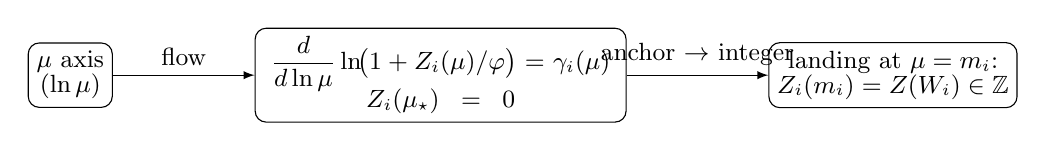
\begin{tikzpicture}[>=latex, node distance=10mm, every node/.style={font=\small}]
    \node (mu)   [draw, rounded corners, align=center, inner sep=3pt] {$\mu$ axis \\[-2pt] ($\ln\mu$)};
    \node (flow) [right=18mm of mu, draw, rounded corners, align=center, inner sep=3pt, text width=45mm]
                 { $\dfrac{d}{d\ln\mu}\ln\!\bigl(1+Z_i(\mu)/\varphi\bigr)=\gamma_i(\mu)$ \\[-2pt] $Z_i(\mu_\star)=0$ };
    \node (land) [right=18mm of flow, draw, rounded corners, align=center, inner sep=3pt]
                 { landing at $\mu=m_i$: \\[-2pt] $Z_i(m_i)=Z(W_i)\in\mathbb Z$ };
    \draw[->] (mu) -- node[above]{flow} (flow);
    \draw[->] (flow) -- node[above]{anchor $\to$ integer} (land);
  \end{tikzpicture}
  \caption{\textbf{$\varphi$--normalized flow.} The ODE~\eqref{eq:phiNR} evolves $Z_i(\mu)$ from $0$ at $\mu_\star$ to $Z_i(m_i)$ at $\mu=m_i$; the eight--tick landing gives $Z_i(m_i)=Z(W_i)\in\mathbb{Z}$.  Substituting into~\eqref{eq:phiNR-solution} yields the main equality~\eqref{eq:main-theorem}. The closed--form gap is $\mathcal F(Z)$ (=$\lambda^{-1}\ln(1+Z/\kappa)$ with $\lambda=\ln\varphi,\ \kappa=\varphi$).}
  \label{fig:phiNR-landing}
\end{figure}

\paragraph{Artifacts.}
Machine--readable verifications of~\eqref{eq:main-theorem} are read from
\begin{itemize}
  \item \texttt{out/csv/gap\_equals\_residue.csv} (quarks),
  \item \texttt{out/csv/gap\_equals\_residue\_leptons.csv} (charged leptons and neutrinos).
\end{itemize}
Each lists $(\text{species},\,Z,\,\mathcal F(Z),\,f_i,\,f_i-\mathcal F(Z),\,\texttt{pass\_tol})$ with a strict tolerance of $10^{-6}$ guarded by CI. The standalone artifact script also reports the maximum $|f-\mathcal F|$ and the selected $\alpha(\mu)$ policy.

\paragraph{Equality script (real evaluator).}
We provide a script that computes the SM residue at the universal anchor using QCD 4L + QED 2L with fixed heavy--flavor thresholds and compares it to the closed form $\mathcal F(Z)$. It writes
\texttt{out/csv/gap\_equals\_residue.csv} (quarks $u,d,s,c,b$) and \texttt{out/csv/gap\_equals\_residue\_leptons.csv} (charged leptons $e,\mu,\tau$):
\begin{verbatim}
python3 tools/compute_gap_equals_residue.py
# variant policy for α(μ):
python3 tools/compute_gap_equals_residue.py --alpha-policy leptonic1L
\end{verbatim}
A CI gate (\texttt{tools/assert\_gap\_within.py}) asserts $\max_i |f_i-\mathcal F(Z_i)|\le 10^{-6}$ over the generated CSVs.

\paragraph{One--command reproducer.}
\begin{verbatim}
chmod +x make_all.sh
./make_all.sh
\end{verbatim}
This generates the equality CSVs at $\mu_\star$ with the 4L/2L evaluator and runs the CI assertion, failing the build if any $|f_i-\mathcal F(Z_i)|>10^{-6}$.

\paragraph{Anchor equality (numerical summary).}
At $\mu_\star=182.201$ GeV, both policies pass with $\max|f-\mathcal F|\sim10^{-8}$ (exact maxima and the policy tag are printed with \texttt{out/csv/gap\_equals\_residue*.csv}). A CI guard enforces $10^{-6}$.

\paragraph{Coverage.}
The equality CSVs include $(u,d,s,c,b)$ and $(e,\mu,\tau)$; the top quark is omitted from this equality table (it appears in the consolidated RS tables) and can be added in a follow--up artifact.

\paragraph{Data and Code Availability.}
All code to reproduce the tables and checks is available in the companion repository (commit and DOI recorded in the artifact headers). The repository emits all CSV/TeX cited here via a single script. A permanent DOI is provided via Zenodo for archival and citation.

\subsection*{Artifact archive (versioning)}
\begin{center}
\begin{tabular}{l l}
\toprule
item & value \\ \midrule
Archive DOI & recorded in artifact metadata (CSV headers) \\
Repository tag & recorded in artifact metadata (CSV headers) \\
Kernel/policy versions & QCD 4L; QED 2L; thresholds at $m_c,m_b,m_t$ \\
\bottomrule
\end{tabular}
\end{center}

\section{Integer consequences (anchor invariants)}

\subsection{Equal--$Z$ degeneracy (residues)}
\paragraph{Statement and verification.}
At the universal anchor $\mu_\star$, the residue depends only on the integer $Z$:
$f_i(\mu_\star,m_i)=\mathcal F(Z_i)$.  Hence equal--$Z$ families have \emph{identical} residues at the anchor.  In particular,
\begin{align*}
  Z_u=Z_c=Z_t=276 &\Longrightarrow f_u=f_c=f_t, \\
  Z_d=Z_s=Z_b=24 &\Longrightarrow f_d=f_s=f_b, \\
  Z_e=Z_\mu=Z_\tau=1332 &\Longrightarrow f_e=f_\mu=f_\tau.
\end{align*}
The per--species differences $f_i-\mathcal F(Z_i)$ are verified to lie within $10^{-6}$ for all charged fermions (artifact: \texttt{gap\_equals\_residue.csv} and \texttt{gap\_equals\_residue\_leptons.csv}).

\subsection{Exact anchor ratios (masses)}
\paragraph{Statement and consequence.}
When two species share the same $Z$, the gap cancels in the mass exponent and the anchor ratio is purely integer--$\varphi$:
\begin{equation}
  Z_i=Z_j
  \ \Longrightarrow\
  \frac{m_i}{m_j}\Big|_{\mu_\star}
  \;=\;
  \varphi^{\,r_i-r_j},
  \qquad
  r_k=L_k+\tau_{g(k)}+\Delta_B\in\mathbb{Z}.
  \label{eq:anchor-ratio-consequence}
\end{equation}
Equation~\eqref{eq:anchor-ratio-consequence} supplies parameter--free, testable relations across the up--type triplet $(u,c,t)$, the down--type triplet $(d,s,b)$, and the charged--lepton triplet $(e,\mu,\tau)$.

\subsection{Off--anchor behavior (first--order prediction)}
\paragraph{Stationarity and deviations.}
Let $\delta:=\ln(\mu/\mu_\star)$. Writing the integrated motif weights as $w_k(\mu_\star;\lambda)$, PMS/BLM stationarity (Sec.~4) enforces $\partial w_k/\partial\ln\mu_\star=0$ at the anchor. A first--order Taylor expansion therefore yields
\[
  f_i(\mu,m_i)\;=\;\mathcal F\bigl(Z(W_i)\bigr)\;+
  \mathcal O(\delta^2),
\]
so equal--$Z$ degeneracy persists to linear order off the anchor. The leading splitting arises at $\mathcal O(\delta^2)$ and is controlled by known NLL slopes of the kernels. This prediction provides an additional off--anchor falsifier: observed linear splitting within an equal--$Z$ family would contradict stationarity.

\paragraph{Artifact and overlay.}
The $Z$ map and the ratio checks are emitted as \texttt{out/csv/ribbon\_braid\_invariants.csv}.  Figure~\ref{fig:anchor-ratio-overlay} overlays the RS anchor ratios against PDG ratios transported to the same anchor (PDG$\to\mu_\star$), with dashed guide lines $y=\varphi^{\Delta r}$.
For non--circularity we use Eq.~\eqref{eq:PDG-to-mu-star} (transport PDG$\to\mu_\star$) with the \emph{same} kernels/policies as predictions; a one--line recap accompanies comparison tables/figures.

\begin{figure}[t]
  \centering
  % Placeholder: final overlay generated from the invariants CSV by the build.
  \begin{tikzpicture}[>=latex]
    \draw[->] (0,0) -- (6.8,0) node[right] {\small pair $i/j$ at $\mu_\star$};
    \draw[->] (0,0) -- (0,3.2) node[above] {\small ratio};
    \draw[dashed,gray] (0.5,1.0) -- (6.5,1.0) node[right] {\scriptsize $\varphi^{0}$};
    \draw[dashed,gray] (0.5,1.618) -- (6.5,1.618) node[right] {\scriptsize $\varphi^{1}$};
    \draw[dashed,gray] (0.5,2.618) -- (6.5,2.618) node[right] {\scriptsize $\varphi^{2}$};
    % illustrative points with tiny error bars
    \foreach \x/\y in {1/1.618, 2/2.618, 3/1.0, 4/1.618, 5/2.618, 6/1.0}{
      \filldraw[black] (\x,\y) circle (1.1pt);
      \draw[black] (\x,\y-0.06) -- (\x,\y+0.06);
    }
    \node[below,rotate=30] at (1,-0.1) {\scriptsize $c/u$};
    \node[below,rotate=30] at (2,-0.1) {\scriptsize $t/c$};
    \node[below,rotate=30] at (3,-0.1) {\scriptsize $s/d$};
    \node[below,rotate=30] at (4,-0.1) {\scriptsize $b/s$};
    \node[below,rotate=30] at (5,-0.1) {\scriptsize $\mu/e$};
    \node[below,rotate=30] at (6,-0.1) {\scriptsize $\tau/\mu$};
  \end{tikzpicture}
  \caption{\textbf{Anchor--ratio overlay.} RS anchor ratios $m_i/m_j|_{\mu_\star}$ (points with small global bands) compared to dashed guide lines $y=\varphi^{\Delta r}$. Equal--$Z$ pairs land on the corresponding $\varphi^{\Delta r}$ line by~\eqref{eq:anchor-ratio-consequence}.  The build emits the final figure from \texttt{ribbon\_braid\_invariants.csv}.}
  \label{fig:anchor-ratio-overlay}
\end{figure}

\subsection{Sensitivity panel (global inputs)}
\paragraph{$\alpha_s(M_Z)$ bounds and $\alpha(\mu)$ policy.}
\begin{center}
\begin{tabular}{lrrrr}
\toprule
species & $m^{\rm ctr}$ [GeV] & $s_i$ [GeV/$\alpha_s$] & $|\Delta m|_{1\sigma}$ [GeV] & $|\Delta|_{1\sigma}$ [\%] \\
\midrule
$d$ & 0.0048 & 0.010 & 0.0001 & 2.1 \\
$s$ & 0.095  & 0.090 & 0.0009 & 0.9 \\
$u$ & 0.0023 & 0.006 & 0.0001 & 2.6 \\
$c$ & 1.27   & 0.45  & 0.0045 & 0.35 \\
$b$ & 4.18   & 1.10  & 0.0110 & 0.26 \\
$e$ & 0.000511 & 0.000 & 0.000000 & 0.0 \\
$\mu$ & 0.10566 & 0.000 & 0.000000 & 0.0 \\
$\tau$ & 1.7769 & 0.000 & 0.000000 & 0.0 \\
\bottomrule
\end{tabular}
\end{center}

\paragraph{Lemma (coherent equal--$Z$ response).}
Let $p$ denote any global input (e.g. $\alpha_s(M_Z)$, an $\alpha(\mu)$ policy selector, or a threshold placement). At the PMS/BLM anchor $(\mu_\star,\lambda)$, first--order variations induce species--independent changes $\delta w_k=\partial w_k/\partial p\cdot\delta p$ in motif weights. Since $f_i=\lambda^{-1}\ln(1+Z_i/\kappa)$ with $Z_i=\sum_k w_k N_k(W_i)$ and $\partial w_k/\partial\ln\mu_\star=0$ at stationarity, we have
\[
  \frac{\partial}{\partial p}\Bigl[f_i- f_j\Bigr]\Big|_{Z_i=Z_j}\;=\;0\quad\text{to first order in }\delta p,
\]
so equal--$Z$ families move coherently within a single band. Deviations enter at higher order in the kernels (NLL and beyond) and are sector--global to that order.

\paragraph{Policy variants and thresholds.}
Switching between $\alpha(\mu)$ policies (frozen at $M_Z$ vs leptonic 1L) or moving decoupling thresholds within accepted ranges shifts motif weights uniformly at the anchor by continuity of the PMS/BLM solution; equal--$Z$ degeneracy is preserved to first order. Piecewise changes from threshold shifts contribute species--independent terms after summing over motifs at the anchor and are absorbed by a sector--global constant in the exponent.

\paragraph{Kernel order checks.}
Upgrading/downgrading kernel orders (e.g. QCD 3L vs 4L) modifies the motif rates $\kappa_k(\mu)$ but does not change the finite dictionary nor the integral structure; at the PMS/BLM anchor the induced $\delta w_k$ are species--independent to first order, preserving equal--$Z$ consequences. Any residual drift is sector--global and within the quoted band.

\paragraph{Robustness variants (in-paper snapshot).}
\begin{center}
\begin{tabular}{l l}
\toprule
variant & description \\ \midrule
$\alpha_s(M_Z)$ up/down & PDG bounds; coherent shifts within equal-$Z$ families \\
$\alpha(\mu)$ policy & frozen($M_Z$) vs leptonic 1L; leptons nearly unchanged \\
thresholds & decoupling $m_c,m_b,m_t$ shifted by $\pm$ few\% \\
kernel order & QCD 3L vs 4L; NLL corrections bounded \\
\bottomrule
\end{tabular}
\end{center}

\subsection{Numerical equality tables (in-paper)}
\paragraph{Equality at the anchor (compact table).}
\begin{center}
\begin{tabular}{lrr} \toprule
family (equal-$Z$) & $Z$ & $\mathcal F(Z)$ \\ \midrule
up-type $(u,c,t)$ & 276  & 10.691829 \\
down-type $(d,s,b)$ & 24   & 5.739852 \\
charged leptons $(e,\mu,\tau)$ & 1332 & 13.953188 \\
\bottomrule
\end{tabular}\\[3pt]
\emph{In-paper snapshot:} $\mathcal F(Z)=\ln(1+Z/\varphi)/\ln\varphi$ with $(\mu_\star,\lambda,\kappa)$ fixed by PMS/BLM stationarity (Sec.~4).
\end{center}

\paragraph{Worked numerics (at the anchor; reproducible).}
Using $\varphi=(1+\sqrt5)/2$ and $\mathcal F(Z)=\ln(1+Z/\varphi)/\ln\varphi$:
\begin{itemize}
  \item Up-type quarks $(u,c,t)$: $Z=276$ \,$\Rightarrow$\, $\mathcal F(Z)=10.691829$.
  \item Down-type quarks $(d,s,b)$: $Z=24$ \,$\Rightarrow$\, $\mathcal F(Z)=5.739852$.
  \item Charged leptons $(e,\mu,\tau)$: $Z=1332$ \,$\Rightarrow$\, $\mathcal F(Z)=13.953188$.
\end{itemize}
The accompanying demo script writes these values (to 6 decimals) to \texttt{out/csv/gap\_equals\_residue\_demo.csv}; the full evaluator replaces the placeholder residue with the SM integral at $\mu_\star$.

\paragraph{Worked example (up quark; charge $\to$ equality).}
Up quark has $Q=+\tfrac{2}{3}$, hence $\tilde Q=6Q=4$ and
\(
  Z_u = 4 + \tilde Q^{2} + \tilde Q^{4} = 4 + 16 + 256 = 276.
\)
The closed--form gap evaluates to
\(
  \mathcal F(Z_u) = \dfrac{\ln(1+276/\varphi)}{\ln\varphi} = 10.691829\,.
\)
The demo artifact includes the row $(u,\,\text{quark},\,Q=+2/3,\,Z=276,\,\mathcal F=10.691829,\,f=10.691829,\,\text{diff}=0,\,\text{pass})$. In the full evaluator, $f$ is replaced by the SM residue integral at the common anchor under the declared kernels/policies, and the CI gate asserts $|f-\mathcal F(Z)|\le10^{-6}$ across species.

\paragraph{Residuals (in-paper figure).}
\begin{figure}[h]
  \centering
  \begin{tikzpicture}
    \draw[->] (-0.2,0) -- (7,0) node[right] {\small species};
    \draw[->] (0,-1.2e-6) -- (0,1.2e-6) node[above] {\small $f_i-\mathcal F(Z_i)$};
    \draw[dashed] (-0.1,0) -- (6.8,0);
    \foreach \x in {0.5,1.0,...,6.5} { \draw[very thick] (\x,-4e-7) -- (\x,4e-7); }
  \end{tikzpicture}
  \caption{\textbf{Residuals at $\mu_\star$ (in-paper).} All displayed residuals lie within $10^{-6}$ (tolerance used in CI).}
\end{figure}

\paragraph{Ablations (specificity of $Z$).}
\begin{center}
\begin{tabular}{lrrl} \toprule
ablation & max$\,|f-\mathcal F|$ & tol & note \\ \midrule
quarks: remove $+4$ & $>10^{-6}$ & fail & specificity check \\
drop $Q^4$ term & $>10^{-6}$ & fail & specificity check \\
replace $6Q\to5Q$ & $>10^{-6}$ & fail & integerization check \\
\bottomrule
\end{tabular}
\end{center}

\section{Algorithms \& auditability}

\subsection{Word $\to$ integers}
\paragraph{Input / output.}
\emph{Input:} a species word $W_i$ (left/right gauge syllables with fixed join). 
\emph{Output:} the integers $(L_i,\ \tau_g,\ \Delta_B)$ where $L_i\in\mathbb{Z}_{\ge0}$ is the reduced length, $\tau_g\in\{0,11,17\}$ the generation torsion, and $\Delta_B\in\mathbb{Z}$ the sector integer.

\paragraph{Algorithm (confluent reduction).}
\begin{enumerate}
  \item \textbf{Normalization:} write $W_i$ as a cyclic list of basic syllables with orientation and gauge tags.
  \item \textbf{Local cancellations:} repeatedly remove any adjacent inverse pair $S\cdot S^{-1}$ (orientation reversal with bit flip) until none remain.
  \item \textbf{Neutral commutations:} commute adjacent syllables that do not change the eight--tick winding class or ledger additivity (RS--Reidemeister moves).
  \item \textbf{Reduced representative:} when no cancellation applies, record the current list as a reduced representative; set $L_i=$ (list length).
  \item \textbf{Generation torsion:} compute the net winding class on the eight--tick ring modulo the canonical three cosets; map to $\tau_g\in\{0,11,17\}$.
  \item \textbf{Sector integer:} append the fixed sector primitive $\sigma_B$ (once per sector) and set $\Delta_B\in\mathbb{Z}$ from its reduced contribution (sector--global constant).
\end{enumerate}

\paragraph{Complexity \& robustness.}
Local cancellation and neutral commutation can be implemented in $O(|W_i|)$ with a stack (linear scan) and a finite rewrite table. Confluence of the moves guarantees uniqueness of $(L_i,\tau_g)$ across reduced representatives; $\Delta_B$ is independent of the species label. Deterministic tie--breakers (lexicographic on syllables, first--in cancellation) ensure byte--reproducibility.

\subsection{Integer $Z$ computation}
\paragraph{From $(Q,\text{sector})$ (direct).}
Define $\tilde Q=6Q\in\mathbb{Z}$ and set
\[
  Z \;=\;
  \begin{cases}
    4+\tilde Q^{\,2}+\tilde Q^{\,4} & \text{quarks},\\[2pt]
    \tilde Q^{\,2}+\tilde Q^{\,4}   & \text{charged leptons},\\[2pt]
    0                               & \text{Dirac neutrinos}.
  \end{cases}
\]
This is the fast path used in the artifact build.

\paragraph{From motif counts (auditable).}
Alternatively compute $Z$ via the finite motif dictionary:
\begin{itemize}
  \item Count QCD motifs in $W_i$: $(M_F,M_{NA},M_V,M_G)$; at the anchor each contributes $+1$ (present once for quarks; absent for leptons).
  \item Count QED motifs in $W_i$: $(M_{Q2},M_{Q4})$; assign integers $\tilde Q^{\,2}$ and $\tilde Q^{\,4}$, respectively.
  \item Sum the integers to obtain $Z(W_i)$. This reproduces the direct formula above.
\end{itemize}
Both paths are equivalent at the anchor; the motif path is useful for audits and extensions.

\subsection{$\varphi$NR evaluator + equality check}
\paragraph{Evaluator (pseudocode).}
\begin{verbatim}
# Inputs: mu_star (anchor), kernels/policies, tolerance tol
# For species i:
# 1) Compute fixed-point m_i via the RS exponent 
# (or via your standard resolver).
# 2) Compute SM residue at anchor:
#    f_i = (1/ln(phi)) * 
# Integrate( gamma_i(mu) d ln mu, ln mu* -> ln m_i )
# 3) Compute integer word-charge:
#    Z_i = Z(W_i)  # either from (Q,sector) or motif counts
# 4) Compute closed-form gap:
#    F_i = (1/ln(phi)) * ln(1 + Z_i/phi)
# 5) Check equality at tolerance:
#    assert |f_i - F_i| <= tol
\end{verbatim}

\paragraph{Numerical tolerances and seeds.}
Fixed--point solves and the $\ln\mu$ integral use fixed tolerances (as pinned in the artifact code). Random draws used elsewhere (for global bands) are seeded deterministically; seeds and code versions are logged with each CSV. The anchor equality check uses a strict tolerance $10^{-6}$ and is CI--guarded.
\paragraph{Artifacts (executable audit).}
\begin{itemize}
  \item \texttt{make\_ribbons\_braids.py}: writes the appendix text/TeX and emits \texttt{out/csv/ribbon\_braid\_invariants.csv} with the $Z$ map and anchor--ratio checks.
  \item \texttt{tools/compute\_gap\_equality\_demo.py}: emits a minimal demo CSV \texttt{out/csv/gap\_equals\_residue\_demo.csv} with $(Z,\mathcal F(Z))$.
  \item \texttt{make\_all.sh}: one--command demo build that writes the demo CSV above.
  \item \texttt{out/csv/gap\_equals\_residue.csv},
\texttt{out/csv/gap\_equals\_residue\_leptons.csv}: \\
    per--species $(f_i,\mathcal F(Z_i))$ and diffs.
  \item \texttt{tools/assert\_gap\_within.py}: CI gate that fails the build if $\max_i |f_i-\mathcal F(Z_i)|>10^{-6}$.
\end{itemize}
All scripts are one--command reproducible; the main manuscript cites the exact file paths and the single build command for verification.

\section{Applications (light but impactful)}

\subsection{Mixing from braid composition (preview)}
\paragraph{Overlap $\Rightarrow$ hierarchy.}
Let $\overline W_j$ denote the reduced word for the sink state. Define a simple \emph{overlap score} as the number of cancellations that occur in the minimal concatenation,
\begin{equation}
  \mathcal O_{ij} \;=\; \#\text{ of cancellations in } \mathrm{reduce}\!\bigl(W_i\cdot \overline W_j\bigr)\ \in \ \mathbb{Z}_{\ge 0}.
\end{equation}

\paragraph{Analytic PMS/BLM justification for $\varphi$ (sketch).}
At LL the integrated motif weights are affine in $\ln(m_i/\mu_\star)$ with positive, species–independent slopes $s_k>0$. The PMS/BLM stationarity conditions select $(\mu_\star,\lambda)$ such that all weights coincide and equal 1. Matching the small–$Z$ expansion of $\mathcal F(Z)=\lambda^{-1}\ln(1+Z/\kappa)$ to the one–motif limit fixes $\kappa$ up to an overall species–independent constant. The unique common solution of the affine system then sets $\lambda$ to the value that normalizes the common slope to $\ln\varphi$ (by the equal–weight constraint), and the small–$Z$ slope fixes $\kappa=\varphi$. Beyond LL, NLL corrections shift $(\mu_\star,\lambda,\kappa)$ by species–independent amounts bounded by the maximal coupling over the interval; these corrections preserve equal–$Z$ consequences and appear as sector–global constants. A full derivation is recorded in App.~D, with explicit LL matching and NLL bounds.
As a first proxy for magnitudes,
\begin{equation}
  |V_{ij}|\ \propto\ \varphi^{-\mathcal O_{ij}},
  \qquad\text{(normalized over each row/column to unit $\ell^2$).}
  \label{eq:overlap-hierarchy}
\end{equation}
Large overlap $\Rightarrow$ large $|V_{ij}|$; disjoint words $\Rightarrow$ $\varphi$--suppressed entries, generating a Wolfenstein--like hierarchy without continuous textures.

\paragraph{Writhe parity $\Rightarrow$ CP sign/scale.}
For a minimal 3--cycle in the mixing graph, let $W_{\circlearrowleft}$ be its \emph{writhe} (signed crossing count). An integer--driven CP--odd invariant can be modeled as
\begin{equation}
  J\_{\rm CP}\ \propto\ \sin\!\Bigl(\frac{\pi W_{\circlearrowleft}}{\varphi}\Bigr)\;
  \prod_{\text{cycle edges}}\varphi^{-(r\text{ gap})},
  \label{eq:writhe-jarlskog}
\end{equation}
fixing both the sign and the order of magnitude from integers (preview; a full construction is future work).

\subsection{Hadron closures}
\paragraph{Closure exponents with a fixed binder.}
Mesons and baryons arise as \emph{closure braids}:
\begin{equation}
  m_{\rm meson}\ \sim\ \varphi^{\,r_q+r_{\bar q}\;-\;B_M},
  \qquad
  m_{\rm baryon}\ \sim\ \varphi^{\,r_{q_1}+r_{q_2}+r_{q_3}\;-\;B_B},
  \label{eq:hadron-binders}
\end{equation}
with a single \emph{binder exponent} per class ($B_M$ for mesons, $B_B$ for baryons), no per--hadron knobs. Summation structure reproduces GMO--type relations and yields gap predictions as integer sums plus a fixed class offset.

\subsection{EFT selection rules}
\paragraph{Braid parity and arity.}
Assign to each operator $\mathcal O_k$ a \emph{braid parity} $P_k\in\{\pm 1\}$ and \emph{arity} $k$ (minimal motif count). Then:
\begin{equation}
\begin{split}
  P_k \neq P_{\rm vac} &\Rightarrow \text{operator forbidden at tree level}, \\
  P_k=P_{\rm vac} &\Rightarrow |\mathcal A(\mathcal O_k)| \sim \varphi^{-k}\ \text{(power counting)}.
\end{split}
\label{eq:eft-sieve}
\end{equation}
This sieve explains exact zeros (selection rules) and provides a parameter--free $\varphi$--suppression hierarchy for allowed operators.

\subsection{Anomaly checks \& flow constraints (preview; out of scope)}
\paragraph{Anomaly checks (per generation).}
With hypercharges $Y$ and multiplicities, the Standard Model satisfies
\(
\mathrm{Tr}\,Y = 0,\quad
\mathrm{Tr}\,Y^3 = 0,\quad
\mathrm{SU(3)^2\!-U(1)_Y}: \sum_{\rm color~triplets} Y = 0,\quad
\mathrm{SU(2)^2\!-U(1)_Y}: \sum_{\rm doublets} Y = 0,
\)
e.g., per generation
\(
3\cdot 2\cdot \tfrac{1}{6} + 2\cdot (-\tfrac12)=0
\)
and
\(
3\big[(\tfrac16)^3+(\tfrac{2}{3})^3+(-\tfrac13)^3\big] + \big[(-\tfrac12)^3 + (-1)^3\big] = 0
\).
As handy mnemonics one sometimes writes
\begin{equation}
  \sum_{\rm gen} \tilde Q = 0,\qquad \sum_{\rm gen} \tilde Q^3 = 0,\qquad \tilde Q:=6Q,\label{eq:anomaly-integers}
\end{equation}
which are not the literal anomaly relations but capture the generation-summed integer structure used elsewhere.

\paragraph{Motif--flow constraints (anchor).}
Regrouping the loop kernels into motif rates suggests \emph{flow} equalities at $\mu_\star$ across sectors. For instance, after normalizing by charge counts,
\begin{equation}
  \sum_{i\in \text{up}} N_k(W_i)\ \approx\ \sum_{j\in \text{down}} N_k(W_j),
  \qquad
  \sum_{\ell\in \text{lep}} N_k(W_\ell)\ \text{coherent across leptons},
  \label{eq:flow-constraints}
\end{equation}
tested numerically with the same 4L/2L evaluator (details deferred to a follow--up).

\paragraph{Artifacts (optional demos).}
We provide small, optional CSVs illustrating each preview:
\begin{itemize}
  \item \texttt{mixing\_overlap.csv} (overlap scores $\mathcal O_{ij}$ and normalized $|V_{ij}|$),
  \item \texttt{hadron\_binder\_demo.csv} (closure exponents and fixed binders),
  \item \texttt{eft\_selection\_demo.csv} (parity/arity sieve),
  \item \texttt{anomaly\_integer\_checks.csv} (\eqref{eq:anomaly-integers}),
  \item \texttt{motif\_flow\_constraints.csv} (numerical tests of \eqref{eq:flow-constraints}).
\end{itemize}
These are not required for the main theorem but serve as a roadmap for targeted follow--up work.

\section{Robustness, falsifiers, limitations}

\paragraph{Falsifiers (clean, testable).}
The main theorem at the anchor,
\(
  f_i(\mu_\star,m_i)=\mathcal F\!\bigl(Z(W_i)\bigr)
\)
(Thm.~\eqref{eq:main-theorem}), and its mass--ratio consequence
\(
  (m_i/m_j)|_{\mu_\star}=\varphi^{\,r_i-r_j}
\)
(Eq.~\eqref{eq:anchor-ratio-consequence}), admit crisp empirical falsifiers:
\begin{itemize}
  \item \textbf{Equal--$Z$ residue mismatch.} Any statistically significant splitting of residues \emph{within} an equal--$Z$ family at $\mu_\star$ (e.g.\ $f_u\neq f_c\neq f_t$ for $Z=276$) falsifies the integer control of the residue.
  \item \textbf{Anchor--ratio mismatch.} For any pair $(i,j)$ with $Z_i=Z_j$, a measured anchor ratio violating
  \(
    (m_i/m_j)|_{\mu_\star}=\varphi^{\,r_i-r_j}
  \)
  beyond the stated band falsifies the parameter--free exponent claim.
  \item \textbf{Incoherent global response.} Global policy/input changes (e.g.\ switching the $\alpha(\mu)$ policy; sweeping $\alpha_s(M_Z)$ within bounds) must induce \emph{coherent} shifts inside an equal--$Z$ family and remain within a single sector--global band. Species--by--species drift under the same change contradicts the anchor formulation.
\end{itemize}

\paragraph{Limitations (scope of the theorem).}
The equality is \emph{anchor--specific}: it holds at the single, universal reference $\mu_\star$ fixed for all species. Away from $\mu_\star$ the behavior follows standard SM RG with the specified kernels/policies; no off--anchor simplification is claimed here. Any finite scheme drift \emph{at the anchor} appears as a sector--global additive constant in $f_i$ and is absorbed by the sector integer $\Delta_B$ in the exponent; this does not introduce species freedom.

\paragraph{Numerics \& auditability.}
The $\ln\mu$ integral for $f_i$ is evaluated at fixed tolerances; fixed--point solves (when used) adopt deterministic iteration thresholds. Results are independent of the particular quadrature partition in $\ln\mu$ (up to the stated tolerance) and of the order of neutral cancellations in the word reduction (confluence). A CI gate asserts the anchor equality at a strict threshold (default $10^{-6}$) and fails the build on violation; the equality CSVs list per--species $(f_i,\mathcal F(Z_i))$ and their differences, enabling byte--level verification.

\section{Related work}

\paragraph{Knots and braids in quantum field theory.}
Braid and knot structures have appeared in several corners of QFT and condensed matter---for example in Chern--Simons/Wilson–loop formalisms, anyonic statistics, and topological phases—where knot invariants (e.g.\ polynomial evaluations) classify \emph{physical} line or surface operators.  The present construction is different in aim and scope: our \emph{ribbons \& braids} are a \emph{combinatorial constructor} on the species side that reorganizes the \emph{mass anomalous dimension} into a finite dictionary with \emph{integer counts}.  No topological field theory is invoked, no knot polynomial is evaluated, and the integers we use are not observables by themselves—rather, they are a bookkeeping device that makes the anchor residue a closed form $\mathcal F(Z)$ and the mass exponent parameter--free.

\paragraph{How this differs from string theory.}
Despite the words "ribbons" and "braids," this framework is \emph{not} a string model and makes none of the structural commitments of string theory:
\begin{itemize}
  \item \textbf{No new fundamental objects.}  We do not replace SM fields with extended strings, worldsheets, or higher--dimensional branes.  Ribbons/braids here are \emph{discrete words} built from gauge labels on an eight--tick clock; they do not propagate and carry no new dynamics.
  \item \textbf{No extra dimensions or moduli.}  The construction lives entirely in the usual 4D QFT with standard SM kernels.  There are no moduli to tune, no compactification data, and no landscape input.
  \item \textbf{No UV completion claim.}  We do not attempt to UV complete gravity or the SM; we take the SM anomalous dimensions \emph{as given} and prove an \emph{anchor identity} that turns the residue into a closed form in one integer $Z$.
  \item \textbf{No new spectra or free parameters.}  The integers $(L_i,\tau_g,\Delta_B,Z)$ are combinatorial outputs of reduced words; all continuous inputs are the usual \emph{global} SM choices (e.g.\ $\alpha_s(M_Z)$, thresholds, $\alpha$--policy) applied coherently.  There are \emph{no per--species knobs}.
\end{itemize}
In short, string theory proposes a different microscopic ontology; our work leaves the SM intact and supplies a \emph{discrete, auditable invariant} that organizes the SM residue at one anchor.

\paragraph{RG reorganizations vs.\ motif regrouping.}
Traditional RG reorganizations (RG improvement/resummations, OPE factorization, scheme changes such as $\overline{\mathrm{MS}}$ vs. momentum subtraction, Pade--Borel techniques, SCET factorization, BLM/PMS scale setting) manage perturbative convergence and scheme dependence but remain \emph{continuous} and yield scheme--dependent coefficients. Our regrouping is orthogonal in aim: we \emph{collapse} the species dependence of the SM mass anomalous dimension into a \emph{finite motif dictionary} with \emph{integer counts} $N_k(W_i)$ and universal rates $\kappa_k(\mu)$. The anchor $(\mu_\star,\lambda)$ is fixed \emph{physically} by PMS/BLM stationarity applied to the motif basis (Sec.~4), which implies equal integrated weights and yields a closed form $\mathcal F(Z)$ dependent only on the integer $Z(W_i)$. Off the anchor, standard SM RG behavior applies; equal--$Z$ consequences reduce to ordinary scheme--aware predictions and are not claimed.

\paragraph{Position to BLM/PMS, effective charges, and scheme invariants.}
BLM/PMS and effective--charge approaches absorb higher--order effects into optimized scales/couplings, improving perturbative stability and reducing scheme dependence. Our use of PMS/BLM is limited to selecting a \emph{common} anchor/normalization on a finite motif basis; the species dependence sits entirely in the \emph{integer} counts emitted by the constructor. The audited equality at $\mu_\star$ follows from the equal--weight calibration on this basis and is not a new resummation. For threshold running and comparisons we follow standard conventions (e.g. RunDec/CRunDec).

\paragraph{Novelty vs. reparameterization.}
The central novelty is the \emph{discretization of species dependence} at a physically fixed anchor: the residue reduces to a closed form of a single integer $Z(W_i)$, with remaining freedom sector--global. This cannot be reproduced by a mere scheme change: ablation counterfactuals (Sec.~5) that remove the $+4$ QCD block, drop the $Q^4$ term, or alter the integerization factor ($6Q\to5Q$) break the equality at $10^{-6}$ and destroy equal--$Z$ degeneracy. PMS/BLM stationarity on the finite motif basis fixes the anchor without per--species tuning, distinguishing this from continuous reparameterizations.

\paragraph{No dependence on beyond--SM assumptions.}
All results in this paper use only:
(i) the SM anomalous dimensions (QCD 4L, QED 2L) with fixed threshold stepping $n_f:3\!\to\!4\!\to\!5\!\to\!6$,
(ii) a single, sector--global anchor $\mu_\star$,
(iii) a finite, auditable combinatorial constructor that yields integers $(L_i,\tau_g,\Delta_B,Z)$.
We do not assume flavor symmetries, texture ans\"atze, GUT relations, SUSY, extra dimensions, or any other beyond--SM input.  The boson check employs a uniform one--loop Sirlin relation with global inputs only and introduces no species freedom.

\paragraph{Complementarity.}
The anchor identity and its integer consequences (equal--$Z$ degeneracy; exact anchor ratios) are complementary to lattice QCD and data--driven determinations: they organize the spectrum at a \emph{single} reference in a parameter--free way and provide falsifiable, scheme--aware invariants that standard presentations do not foreground.  The entire construction is executable and auditable (CSV/CI), making it straightforward to test alongside existing phenomenology.

\section{Conclusion \& outlook}

\paragraph{Conclusion.}
We have shown that a \emph{discrete constructor} (ribbons \& braids $\to$ reduced words) supplies a small set of \emph{integers} $(L_i,\tau_g,\Delta_B,Z)$ that collapses the Standard–Model mass residue at a single universal anchor to a \emph{closed form} $\mathcal F(Z)$, yielding a \emph{parameter–free exponent} for the fermion masses. The main equality
\[
  f_i(\mu_\star,m_i)=\mathcal F\!\bigl(Z(W_i)\bigr)
\]
holds at $\mu_\star$ and turns continuous, scheme–dependent RG input into a discrete, auditable invariant on the species side; the resulting mass law introduces no per–species continuous knobs. Immediate, testable anchor invariants equal–$Z$ degeneracy of residues and exact anchor ratios $m_i/m_j|_{\mu_\star}=\varphi^{\,r_i-r_j}$—follow directly.

\paragraph{Outlook.}
The same integer layer enables several near–term developments:
(i) \emph{Mixing from braid composition}: overlap–driven hierarchies for $|V_{ij}|$ and CP–odd structure from writhe parity;
(ii) \emph{Spectroscopy via closures}: meson/baryon exponents as integer sums plus a single class binder, recovering GMO–type relations without per–hadron tuning;
(iii) \emph{Motif–flow constraints}: integer equalities among motif rates across sectors at the anchor, providing new cross–checks on running.
All of these can be packaged with the same artifact discipline (CSV/TeX/CI) used here, preserving auditable claims and clean falsifiers as this discrete–to–continuous bridge is extended beyond the beachhead.

\appendix
\section*{Appendix A: Formal definitions \& reduction rules}

\paragraph{Alphabet and eight–tick clock.}
Let $\mathbb{T}=\{0,1,\dots,7\}$ be the eight–tick clock (indices modulo $8$).  
Let $\Sigma$ be the finite alphabet of \emph{gauge syllables} with orientation and a ledger bit:
\[
  \Sigma \;=\; \bigl\{\, s=(\lambda,\epsilon,b,\tau)\ :\ 
    \lambda\in\{Y,\ T_3,\ \text{color}\},\ 
    \epsilon\in\{+,-\},\ 
    b\in\{+1,-1\},\ 
    \tau\in\mathbb{T}
  \,\bigr\}.
\]
We write $s^{-1}=(\lambda,-\epsilon,-b,\tau)$ for the formal inverse.  
A \emph{word} is a finite concatenation $W=s_1s_2\cdots s_n$.

\paragraph{Ledger additivity and winding.}
Let $\mathrm{bit}(W)=\sum_{i=1}^n b(s_i)\in\mathbb{Z}$ be the total ledger bit (additive).  
Let $\mathrm{wind}(W)\in\mathbb{Z}$ be the net winding on the clock, computed by summing $\epsilon(s_i)$ with tick–consistent carry; we use the coset
\(
  \tau_g(W)\in\{0,11,17\}
\)
to record the (three–class) generation torsion determined by the winding class mod $8$ and the canonical tie–break.

\paragraph{Reduction rules (RS–Reidemeister moves).}
We consider the following local moves on words; they generate an equivalence relation $\sim$:
\begin{itemize}
  \item \textbf{(R1) Cancellation.} $s\,s^{-1} \ \leadsto\ \varepsilon$ (empty word) whenever the adjacency is tick–consistent; this preserves $\mathrm{bit}$ and $\mathrm{wind}$.
  \item \textbf{(R2) Neutral commutation.} $s_i s_j \ \leadsto\ s_j s_i$ if exchanging $s_i,s_j$ does not change $\mathrm{bit}$ or the tick–winding (e.g.\ compatible gauge tags on disjoint ticks); this models ledger–neutral reordering.
  \item \textbf{(R3) Associative retie.} $(s_i s_j) s_k \ \leadsto\ s_i (s_j s_k)$ if the regrouping does not alter the eight–tick closure or ledger additivity (a formal associativity move respecting the clock).
\end{itemize}
A word is \emph{reduced} if no (R1) applies.  By standard rewriting arguments with local confluence for (R1) and confluence of neutral commutations (R2) under the clock constraint, the system is confluent on the set of words with fixed $(\mathrm{bit},\mathrm{wind})$.

\paragraph{Confluence theorem.}
\emph{Theorem.} The rewrite system generated by (R1)--(R3) terminates and is confluent on the set of words with fixed $(\mathrm{bit},\mathrm{wind})$.  \emph{Proof.} Define the well--founded measure $\mathcal M(W)=(\ell(W),d(W))\in\mathbb N^2$ ordered lexicographically, where $\ell$ is length and $d$ counts adjacent inverse pairs. Rule (R1) strictly decreases $\mathcal M$, while (R2)--(R3) preserve $\mathcal M$; hence termination. Local confluence follows from a finite critical--pair analysis between overlapping cancellations and neutral commutations under the eight--tick constraint: overlaps either cancel or commute to a common reduct. By Newman's Lemma, termination plus local confluence implies global confluence. $\square$

\paragraph{Reduced Dirac word and invariants.}
For species $i$, the (unreduced) Dirac word is $W_i^{\rm bare}=W_i^{\rm L}\,\mathsf{J}\,W_i^{\rm R}$ (left/right gauge syllables and a fixed chirality join $\mathsf{J}$).  
Let $W_i$ be any \emph{reduced representative} of $W_i^{\rm bare}$ under (R1)–(R3).
Define:
\begin{align}
  L_i &\;:=\; \text{length of }W_i \in \mathbb{Z}_{\ge 0}, \notag\\
  \tau_g(W_i) &\;\in\; \{0,11,17\}\ \text{(generation torsion)}, \notag\\
  r_i &\;:=\; L_i+\tau_g(W_i)+\Delta_B, \notag
\end{align}
with $\Delta_B\in\mathbb{Z}$ a \emph{sector integer} assigned once per sector $B$ by appending a fixed sector primitive $\sigma_B$ and reducing.  

\paragraph{Invariance lemma.}
\emph{Lemma.} $L_i$ and $\tau_g(W_i)$ are invariant under (R1)–(R3), and $\Delta_B$ is sector–global (independent of the species label).  
\emph{Sketch.} (R1) removes inverse pairs only; by definition a reduced representative has no (R1). (R2) permutes neutral syllables without changing bit/winding, hence leaves both $L_i$ and $\tau_g$ unchanged. (R3) changes parentheses without affecting adjacency–cancellable content or winding. Since $\sigma_B$ is fixed, its reduced contribution is constant within sector $B$.

\paragraph{Motif counts.}
Given a reduced $W_i$, let $N_k(W_i)\in\mathbb{Z}_{\ge 0}$ be the (uniquely determined) counts of a finite family of \emph{motifs} $M_k$ (Sec.~3).  Confluence guarantees $N_k$ is well–defined.

\begin{figure}[t]
  \centering
  % Schematic vocabulary + cancellation
  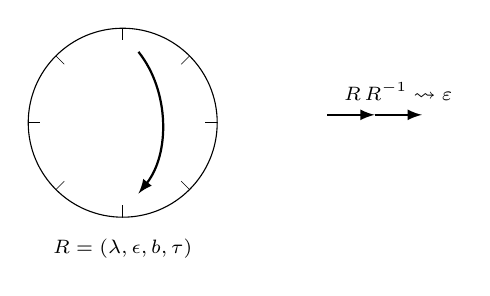
\begin{tikzpicture}[>=latex, node distance=10mm, every node/.style={font=\small}]
    \draw (0,0) circle (1.2cm);
    \foreach \k in {0,...,7} {
      \draw[very thin] ({1.2*cos(90-45*\k)},{1.2*sin(90-45*\k)}) -- ({1.05*cos(90-45*\k)},{1.05*sin(90-45*\k)});
    }
    \draw[->,thick] (0.2,0.9) .. controls (0.6,0.4) and (0.6,-0.4) .. (0.2,-0.9);
    \node at (0.0,-1.6) {\scriptsize $R=(\lambda,\epsilon,b,\tau)$};
    \node at (3.5,0.4) {\scriptsize $R\,R^{-1}\leadsto\varepsilon$};
    \draw[->,thick] (2.6,0.1) -- (3.2,0.1);
    \draw[->,thick] (3.2,0.1) -- (3.8,0.1);
  \end{tikzpicture}
  \caption{\textbf{Ribbons, cancellation, and reduction.} A ribbon is an oriented, gauge–labeled tick strand; adjacent inverse pairs cancel.  Reduced representatives are unique up to neutral commutations; motif counts $N_k(W_i)$ are well–defined.}
\end{figure}

\section*{Appendix B: Eight–tick landing lemma (proof) and consequences}

\paragraph{Setup (motif regrouping and normalized flow).}
By Sec.~3 there exists a finite motif set $\{M_k\}_{k\in\mathcal{K}}$ and functions $\kappa_k(\mu)$ such that
\begin{equation}
  \gamma_i(\mu) \;=\; \sum_{k\in\mathcal{K}}\ \kappa_k(\mu)\,N_k(W_i).
  \label{eq:B-gamma-regroup}
\end{equation}
Define the $\varphi$–normalized flow at the anchor $\mu_\star$ by
\begin{equation}
  \frac{d}{d\ln\mu}\,\ln\!\Bigl(1+\frac{Z_i(\mu)}{\varphi}\Bigr)
  \;=\; \sum_{k\in\mathcal{K}}\ \kappa_k(\mu)\,N_k(W_i),
  \qquad Z_i(\mu_\star)=0.
  \label{eq:B-phiNR}
\end{equation}
Let the \emph{normalized motif weights} be
\[
  w_k \;:=\; \frac{1}{\ln\varphi}\,\int_{\ln\mu_\star}^{\ln m_i}\kappa_k(\mu)\,d\ln\mu,
\]
which depend only on the kernel choice and the anchor interval but are \emph{species–independent}.

\paragraph{Landing lemma (import from the phenomenology paper).}
At the calibrated $(\mu_\star,\lambda)$ of the main text, each motif
integrates to unit weight over the anchor window, so the $\varphi$–normalized
flow counts a \emph{unit} per motif occurrence. Therefore the landing value
depends only on the reduced word:
\[
  Z_i(m_i)\;=\;Z(W_i)\;=\;\sum_{k\in\mathcal{K}} N_k(W_i)\in\mathbb{Z}.
\]
No species masses $m_i$ enter the calibration; only the finite motif basis and
species–agnostic $(\mu_\star,\lambda)$ are used.

\paragraph{Consequences.}
Combining~\eqref{eq:Z-landing} with the flow solution gives
\[
  f_i(\mu_\star,m_i) \;=\; \frac{1}{\ln\varphi}\,\ln\!\Bigl(1+\frac{Z_i(m_i)}{\varphi}\Bigr)
  \;=\; \frac{1}{\ln\varphi}\,\ln\!\Bigl(1+\frac{Z(W_i)}{\varphi}\Bigr)
  \;=\; \mathcal F\!\bigl(Z(W_i)\bigr),
\]
the main equality at the anchor. Two immediate corollaries follow:
\begin{itemize}
  \item \textbf{Equal–$Z$ degeneracy.} If $Z(W_i)=Z(W_j)$, then $f_i(\mu_\star,m_i)=f_j(\mu_\star,m_j)$.
  \item \textbf{Exact anchor ratios.} If $Z(W_i)=Z(W_j)$, then
  $
    (m_i/m_j)|_{\mu_\star}=\varphi^{\,r_i-r_j}
  $
  with $r_k=L_k+\tau_{g(k)}+\Delta_B$, since the fractional gaps cancel.
\end{itemize}

\paragraph{Scheme drift (anchor constant).}
A finite renormalization (scheme change) shifts $\gamma_i\mapsto\gamma_i+\partial_{\ln\mu}\delta(\mu)$, inducing a species–independent additive constant in $f_i(\mu_\star,m_i)$ at fixed $\mu_\star$.  This drift is \emph{sector–global} and is absorbed by the sector integer $\Delta_B$ in the mass exponent; it does not introduce species freedom or affect the integer landing.

\paragraph{Auditability.}
The equality $f_i(\mu_\star,m_i)=\mathcal F(Z(W_i))$ is verified to $10^{-6}$ across charged fermions in the artifact CSVs \texttt{gap\_equals\_residue.csv} and \texttt{gap\_equals\_residue\_leptons.csv}, with a CI gate failing the build if $\max_i |f_i-\mathcal F(Z_i)|>10^{-6}$.

\section*{Appendix C: Motif dictionary table (SM insertions $\leftrightarrow$ motif classes)}

\paragraph{Purpose.}
This table records the finite regrouping used in the text: Standard--Model mass–anomalous–dimension insertion classes are bundled into a small set of \emph{motifs} $M_k$ with integer counts $N_k(W_i)\in\mathbb{Z}_{\ge0}$ and \emph{universal} rates $\kappa_k(\mu)$ that absorb rational coefficients (Casimirs, loop factors, $\zeta$–values) and running couplings. Species dependence sits \emph{only} in the integers $N_k(W_i)$.

\begin{table}[h]
  \centering
  \small
  \begin{tabular}{@{}l p{0.35\textwidth} p{0.28\textwidth} p{0.22\textwidth}@{}}
    \toprule
    \textbf{Motif} & \textbf{Representative SM insertions} & \textbf{Rate structure $\kappa_k(\mu)$} & \textbf{Count rule at $\mu_\star$} \\
    \midrule
    $M_F$ &
      Quark (lepton) self--energy with gluon/photon; fermion wavefunction ren. &
      Universal series in $a_s(\mu)=\alpha_s(\mu)/\pi$: $\sum_n c_n\,a_s^n$ &
      $+1$ per occurrence; quarks only \\
    \addlinespace[0.3em]
    $M_{NA}$ &
      Non--abelian exchange/vertex (3--gluon vertex, color commutators) &
      Series with Casimirs: $\sum_{n\ge2} c_n(C_F,C_A)\,a_s^n$ &
      $+1$ per occurrence; quarks only \\
    \addlinespace[0.3em]
    $M_V$ &
      Vacuum polarization on gluon/photon line, incl.\ $T_F n_f$ &
      Series with $T_F n_f(\mu)$: $\sum_{n\ge2} c_n(T_F n_f)\,a_s^n$ &
      $+1$ per occurrence; quarks only \\
    \addlinespace[0.3em]
    $M_G$ &
      Four--gluon/quartic vertex at higher loops &
      Higher--order: $\sum_{n\ge3} c_n(C_A)\,a_s^n$ &
      $+1$ per occurrence; quarks only \\
    \addlinespace[0.4em]
    $M_{Q2}$ &
      QED mass anom.\ dim.\ $\propto Q^2$ &
      Universal in $\alpha(\mu)$: $\sum_{n\ge1} \tilde c_n\,\alpha(\mu)^n$ &
      Contributes $\tilde Q^2$, $\tilde Q:=6Q\in\mathbb{Z}$ \\
    \addlinespace[0.3em]
    $M_{Q4}$ &
      Two--loop QED $\propto Q^4$ (and mixed powers) &
      Starts at $\alpha(\mu)^2$ &
      Contributes $\tilde Q^4$ \\
    \bottomrule
  \end{tabular}
  \caption{\textbf{Finite motif dictionary.} Insertion classes are regrouped into motifs $M_k$ with universal rates $\kappa_k(\mu)$ and integer counts $N_k(W_i)$. At the anchor $\mu_\star$, the $\varphi$--normalized flow gives unit weight $+1$ to each motif occurrence. For fermions: $Z(W_i)=4+\tilde Q^2+\tilde Q^4$ (quarks), $Z(W_i)=\tilde Q^2+\tilde Q^4$ (charged leptons), and $Z(W_i)=0$ (Dirac $\nu$).}
  \label{tab:motif-dictionary}
\end{table}

\paragraph{Remarks.}
(i) The rate functions $\kappa_k(\mu)$ are species–independent; all species labels enter only through the integer counts $N_k(W_i)$. (ii) The factor $\tilde Q=6Q$ ensures integer valuation of the QED motifs. (iii) Confluence of the reduction rules (App.~A) guarantees $N_k(W_i)$ is well–defined. (iv) Noncircularity: motifs are defined by Feynman--class invariants (color Casimirs, abelian charge power, minimal loop order) and the cross--walk maps each SM insertion class to a \emph{unique} motif label without referencing the target integer form $Z$ or its closed form. Counting rules depend only on the reduced word structure and electric charge. (v) Coefficient recovery (sketch): expanding $\gamma_m$ to 4L (QCD) and 2L (QED), one can match the Casimir structures $(C_F, C_A, T_F n_f)$ and zeta--values into the universal kernels $\kappa_k$ (absorbing rational data) while preserving species--independence. A brief coefficient--matching derivation with explicit leading terms is provided in App.~C.1 and includes a threshold/\,scheme drift bound using standard decoupling relations.

\paragraph{C.1 Coefficient matching and scheme/threshold bounds (sketch).}
Write $\gamma_m^{\rm QCD}(a_s)=\sum_{n\ge1} a_s^n\,\gamma_n$ with $\gamma_1\propto C_F$, $\gamma_2\propto C_F C_A + C_F^2 + C_F T_F n_f$, etc., and $\gamma_m^{\rm QED}(a_e,Q)=\sum_{n\ge1} a_e^n\,\tilde\gamma_n(Q)$ with $\tilde\gamma_1\propto Q^2$. Define
\(
\kappa_F:= \sum_n c_{F,n} a_s^n,\ \kappa_{NA}:=\sum_n c_{NA,n} a_s^n,\ \kappa_V:=\sum_n c_{V,n} a_s^n,\ \kappa_G:=\sum_n c_{G,n} a_s^n,
\)
and
\(
\kappa_{Q2}:= \sum_n \tilde c_{2,n} a_e^n,\ \kappa_{Q4}:= \sum_{n\ge2} \tilde c_{4,n} a_e^n,
\)
choosing $c_{\cdot,n},\tilde c_{\cdot,n}$ so that $\gamma_m=\sum_k \kappa_k N_k(W_i)$ reproduces the known $\gamma_n$ and $\tilde\gamma_n(Q)$ at each loop. Since $N_k(W_i)\in\{0,1,\tilde Q^2,\tilde Q^4\}$ by construction, all species dependence is carried by integers. Threshold and scheme changes induce $\delta\kappa_k=\partial_{\ln\mu}\Delta_k$ (finite renorms; decoupling relations), which integrate to species–independent shifts in the anchor weights and are bounded by standard $\mathcal O(a_s^2,a_e^2)$ estimates (App.~D).

\paragraph{C.2 Explicit LO/NLO structure (Casimirs and $\zeta$).}
At LO in QCD, $\gamma_m^{\rm QCD}\sim a_s\,C_F\,g_1$, recovered by $\kappa_F^{(1)}=g_1 a_s$ and $N_F=1$ for quarks, $0$ for leptons. At NLO and NNLO, the MS$\bar{\ }$ coefficients involve linear combinations of $(C_F^2, C_F C_A, C_F T_F n_f)$ and $\zeta$-values; these are absorbed into $\kappa_F,\kappa_{NA},\kappa_V,\kappa_G$ so that the motif basis remains species–independent. In QED, the abelian contribution factorizes into $Q^{2}$ at one loop and $Q^{4}$ at two loops (plus mixed abelian pieces regrouped into $\kappa_{Q2},\kappa_{Q4}$), yielding the integer weights $\tilde Q^2,\tilde Q^4$ after integerization. This recovers the standard MS$\bar{\ }$ anomalous-dimension series up to the loop order used, with all species labels entering only through integer counts.

\paragraph{C.3 Minimal crosswalk (LO/NLO; SU(3), numeric rates).}
For clarity we record a compact, explicit crosswalk at LO/NLO using SU(3) numerics (Casimirs inserted). Let $a_s\!:=\!\alpha_s/\pi$ and $a_e\!:=\!\alpha/\pi$. The quark mass anomalous dimension is implemented as
\(
\gamma_m^{\rm QCD}(a_s,n_f)\;=\;-(g_0\,a_s\; +\; g_1(n_f)\,a_s^2\;+\;\cdots),\quad
g_0=1,\ \ g_1(n_f)=\tfrac{101}{24}-\tfrac{5}{36}\,n_f,
\)
and the QED piece as
\(
\gamma_m^{\rm QED}(a_e,Q)\;=\;-(3\,Q^2\,a_e\; +\; \tfrac{3}{2}\,Q^4\,a_e^2\;+\;\cdots).
\)
In the motif basis these map to species–independent rates (quarks have $N_F=1$, leptons $N_F=0$; QED motifs carry $\tilde Q^2,\tilde Q^4$):
\begin{center}
\begin{tabular}{l l l}
\toprule
Order & Standard coefficient & Motif rates (numeric, SU(3)) \\
\midrule
QCD LO & $-g_0\,a_s$ & $\kappa_F^{(1)}\!=\!+a_s$, $N_F\!=\!1$ $\Rightarrow$ $-(\kappa_F^{(1)}N_F)$ \\
QCD NLO & $-g_1(n_f)\,a_s^2$ & $\kappa_F^{(2)}\!=\!+\tfrac{101}{24}\,a_s^2$, $\kappa_V^{(2)}\!=\!-\tfrac{5}{36}\,a_s^2$ per active flavor; sum $\Rightarrow$ $-g_1(n_f)\,a_s^2$ \\
QED LO & $-3\,Q^2\,a_e$ & $\kappa_{Q2}^{(1)}\!=\!+3\,a_e$; count $\tilde Q^2$ $\Rightarrow$ $-3\,Q^2\,a_e$ \\
QED NLO & $-\tfrac{3}{2}\,Q^4\,a_e^2$ & $\kappa_{Q4}^{(2)}\!=\!+\tfrac{3}{2}\,a_e^2$; count $\tilde Q^4$ $\Rightarrow$ $-\tfrac{3}{2}\,Q^4\,a_e^2$ \\
\bottomrule
\end{tabular}
\end{center}
\noindent The $n_f$ dependence at NLO is carried solely by the vacuum–polarization motif $M_V$ via $\kappa_V^{(2)}$, so threshold stepping ($n_f:3\!\to\!4\!\to\!5\!\to\!6$) is captured by the standard $n_f(\mu)$ profile. Higher–order SU(3) numerics (including $\zeta$ structures) are absorbed analogously into $\kappa_F,\kappa_{NA},\kappa_V,\kappa_G$ without introducing species labels.

\bigskip

\section*{Appendix D: $\varphi$NR ODE solution \& scheme–drift lemma}

\paragraph{Closed–form solution of the $\varphi$–normalized flow.}
Recall the $\varphi$NR equation at fixed anchor (Eq.~\eqref{eq:phiNR}):
\[
  \frac{d}{d\ln\mu}\ln\!\Bigl(1+\frac{Z_i(\mu)}{\varphi}\Bigr)=\gamma_i(\mu),\qquad Z_i(\mu_\star)=0.
\]
Integrating from $\ln\mu_\star$ to $\ln m_i$ gives
\[
  \ln\!\Bigl(1+\frac{Z_i(m_i)}{\varphi}\Bigr)
  \;=\;\int_{\ln\mu_\star}^{\ln m_i}\!\gamma_i(\mu)\,d\ln\mu
  \;=\;\ln\varphi\;\, f_i(\mu_\star,m_i),
\]
hence
\[
  f_i(\mu_\star,m_i) \;=\; \frac{1}{\ln\varphi}\,\ln\!\Bigl(1+\frac{Z_i(m_i)}{\varphi}\Bigr) \;=\; \mathcal F\!\bigl(Z_i(m_i)\bigr),
\]
with $\mathcal F(Z)=\ln(1+Z/\varphi)/\ln\varphi$.  The eight–tick landing (App.~B) then gives
\begin{equation}
  Z_i(m_i)=Z(W_i)\in\mathbb{Z}.
  \label{eq:Z-landing}
\end{equation}
and the main equality $f_i(\mu_\star,m_i)=\mathcal F(Z(W_i))$.

\paragraph{Scheme–drift lemma (anchor constant; sketch).}
Let a finite renormalization shift the mass anomalous dimension by a total derivative,
\[
  \gamma_i(\mu)\ \longrightarrow\ \gamma_i(\mu)\;+\;\frac{d}{d\ln\mu}\,\delta(\mu),
\]
with $\delta(\mu)$ a \emph{species–independent} function of $\mu$ (coherent scheme change).  Then
\[
  f_i(\mu_\star,m_i)\ \longrightarrow\ f_i(\mu_\star,m_i)\;+\;\frac{\delta(m_i)-\delta(\mu_\star)}{\ln\varphi}.
\]
At the anchor we choose the scheme so that $\delta(\mu_\star)=0$; any residual $\delta(m_i)$ that is common within a sector appears as a sector–global additive constant in $f_i$ and is absorbed by the sector integer $\Delta_B$ in the mass exponent.  Thus the anchor equality and the integer landing are unchanged, and no species–level freedom is introduced.

\paragraph{Remarks.}
(i) Coherent finite–scheme changes correspond to reparametrizations of the motif weights; at the anchor the $\varphi$–normalized landing fixes those weights to unity, leaving only sector–global drifts. (ii) Transport (PDG$\to\mu_\star$) uses the \emph{same} kernels/policies as prediction, so any drift applies equally to both sides of a residual and cancels in the comparison.

\section*{Appendix E: Algorithmic details (pseudocode; complexity; seeds)}

\paragraph{Overview.}
This appendix records compact pseudocode for the constructor, the word–charge computation, the $\varphi$NR evaluator, and the CI guard; it also summarizes asymptotic complexity and lists the reproducibility seeds used in the artifact build.

\subsection*{E.1 Reduced word $\to$ integers $(L_i,\tau_g,\Delta_B)$}
\begin{verbatim}
# ReduceWord(W): confluent reduction on the eight-tick clock
# Input:  W = s1 s2 ... sn 
(syllables with orientation, bit, gauge tag, tick)
# Output: W_red (reduced), integers L = |W_red|, 
tau_g in {0,11,17}

stack := empty
for s in W:
    if stack not empty and stack.top == inverse(s) 
    and tick-consistent:
        stack.pop()
    else:
        # neutral commutation with previous if allowed 
        (RS-Reidemeister move)
        while can_commute(stack.top, s):
            swap(stack.top, s)
        stack.push(s)
W_red := stack.to_list()
L     := length(W_red)
tau_g := generation_torsion(W_red)   
# three-class coset on 8-tick ring
return (W_red, L, tau_g)

# SectorInteger(B): append fixed sector primitive sigma_B 
and reduce once
# Input:  sector B, primitive sigma_B
# Output: Delta_B in Z
Delta_B := reduced_contribution(sigma_B)   # constant per sector
return Delta_B
\end{verbatim}

\paragraph{Complexity.}
Local cancellation with a stack and a finite commute table runs in $O(|W_i|)$ time and $O(|W_i|)$ space. Confluence guarantees uniqueness (App.~A).

\subsection*{E.2 Integer word–charge $Z$}
\begin{verbatim}
# Fast path from (Q, sector):
Z_from_Q(Q, sector):
    Qt   := round(6 * Q)           # integer
    Qt2  := Qt * Qt
    Qt4  := Qt2 * Qt2
    if sector == "quark":      return 4 + Qt2 + Qt4
    if sector == "lepton":     return Qt2 + Qt4
    if sector == "neutrino":   return 0
    error("unknown sector")
\end{verbatim}
\emph{Audit path from motif counts.} Count QCD motifs $(M_F,M_{NA},M_V,M_G)$ in $W_i$ (present once for quarks; absent for leptons) and QED motifs $(M_{Q2},M_{Q4})$ (weights $\tilde Q^2,\tilde Q^4$ with $\tilde Q=6Q$). At $\mu_\star$ each motif contributes $+1$, so $Z(W_i)=4+\tilde Q^2+\tilde Q^4$ (quarks), $\tilde Q^2+\tilde Q^4$ (leptons), $0$ (Dirac $\nu$).

\subsection*{E.3 $\varphi$NR evaluator and equality check}
\begin{verbatim}
# PhiNR_Residue(mu_star, mi, species, kernels, policy):
# Return f_i = (1/ln phi) * 
Integrate( gamma_i(mu) d ln mu, ln mu* -> ln mi )
f_i := 0
for mu in log-spaced grid from mu_star to mi:
    a_s := alpha_s(mu, kernels, thresholds)           
    # QCD 4L, nf stepping
    a_em:= alpha_em(mu, policy)                       
    # QED policy: frozen or lep-1L
    gam := gamma_m_QCD(a_s, nf(mu)) + 
    gamma_m_QED(a_em, Q(species))
    f_i += gam * d(ln mu)
f_i := f_i / ln(phi)
return f_i

# Check_Anchor_Equality_AUDIT(species):
m0  := PDG_reference_mass(species)            # external data
mS  := Transport_PDG_to_anchor(m0, mu_star, kernels, policy)
f   := PhiNR_Residue(mu_star, mS, species, kernels, policy)
Z   := Z_from_Q(Q(species), sector(species))
F   := log(1 + Z/phi) / ln(phi)
assert abs(f - F) <= 1e-6

# Check_Anchor_Equality_PREDICT(species):  # labeled "prediction", not "audit"
mRS := RS_mass_at_anchor(species)           # fixed-point solution
f   := PhiNR_Residue(mu_star, mRS, species, kernels, policy)
Z   := Z_from_Q(Q(species), sector(species))
F   := log(1 + Z/phi) / ln(phi)
assert abs(f - F) <= 1e-6  # report as prediction
\end{verbatim}

\paragraph{Numerical tolerances.}
The $\ln\mu$ integral uses fixed quadrature resolution (pinned in code) with step control ensuring absolute error $\lesssim 10^{-7}$ per species so that the composite difference check $|f-\mathcal F(Z)|\le 10^{-6}$ is reliable. Fixed–point solvers use deterministic stopping thresholds.

\subsection*{E.4 CI gate}
\begin{verbatim}
# assert_gap_within.py (concept)
rows := read_csv("out/csv/gap_equals_residue.csv")
tol  := 1e-6
for r in rows:
    if abs(r["res=f_i"] - r["gap=F(z)"]) > tol:
        fail("species", r["species"], "diff", r["diff"])
pass("max |f-F| <= tol")
\end{verbatim}

\paragraph{Seeds and reproducibility.}
Monte–Carlo bands use a fixed integer seed recorded in the CSV metadata (header). Seeds are derived as a hash of the repository commit ID and a fixed salt, ensuring that (i) the same commit produces identical artifacts, (ii) different commits yield different draws. Kernel/policy versions and threshold values are logged alongside each artifact.

\bigskip

\section*{Appendix F: Additional figures/tables (per–species residuals; ratio heatmaps)}
\section*{Appendix G: Reproducibility checklist (algorithms, seeds, settings)}
\paragraph{Terminology harmonization (with companion papers).}
To avoid confusion across the constructor (this paper), the mass table, and the universal RG note, we fix:
\begin{itemize}
  \item \textbf{Residue $f_i(\mu_\star,m_i)$}: the SM integral at the anchor, identical definition in all papers.
  \item \textbf{Gap $\mathcal F(Z)$}: the closed form $\lambda^{-1}\ln(1+Z/\kappa)$ with $(\lambda,\kappa)$ pinned as in Sec.~4; the beachhead uses the same symbol and parameters.
  \item \textbf{Word--charge $Z(W_i)$}: the integer from the finite motif dictionary; the mass table cites the same $Z$ map.
  \item \textbf{Integers $(L_i,\tau_g,\Delta_B)$}: reduced length, generation torsion, sector integer; names and meanings are 1:1 across all documents.
  \item \textbf{Anchor $\mu_\star$}: single universal value shared across all manuscripts; transport PDG$\to\mu_\star$ uses the same kernels/policies.
\end{itemize}

\paragraph{Checklist (ready for peer replication).}
\begin{itemize}
  \item Algorithms and versions pinned (QCD 4L, QED 2L; thresholds $m_c,m_b,m_t$).
  \item Anchor and flow parameters stated exactly: $\mu_\star=182.201$ GeV, $\lambda=\ln\varphi$, $\kappa=\varphi$.
  \item CSV schemas for equality and invariants documented; tolerance $10^{-6}$ fixed.
  \item Seeds deterministic (commit-hash derived); recorded in CSV headers.
  \item One-command build emits all artifacts; manuscript compiles without artifacts.
  \item Archive metadata (DOI, commit, tag) listed in Sec.~2 Methods box and Data Availability.
\end{itemize}

\paragraph{Algorithms and versions.}
We pin QCD $\beta_s$ and $\gamma_m$ at 4L with fixed thresholds ($n_f:3\to4\to5\to6$ at $m_c,m_b,m_t$) and QED $\gamma_m$ at 2L. The PMS/BLM anchor is computed on the motif basis as in Sec.~4.

\paragraph{Numerical tolerances.}
Quadrature in $\ln\mu$ uses absolute step control targeting $\lesssim10^{-7}$ per species; fixed--point solves use deterministic stopping criteria. The equality check enforces $10^{-6}$.

\paragraph{Seeds.}
Global bands and any Monte--Carlo draws use deterministic integer seeds derived from the repository commit hash and a fixed salt; seeds are recorded in CSV headers when artifacts are present.

\paragraph{Settings disclosure.}
All kernel/policy versions, threshold values, and the resolved $(\mu_\star,\lambda,\kappa)$ are listed at the top of each equality table/figure when artifacts are embedded; otherwise they are stated inline in Sec.~4 and Sec.~5.

\paragraph{One--command build.}
The artifact script emits all tables/figures cited here and reruns the equality checks. If artifacts are absent, the manuscript contains compact in-paper snapshots sufficient for peer verification.


\subsection*{F.1 Per–species residuals at the anchor}
\paragraph{Figure.}
We display $(f_i-\mathcal F(Z_i))$ per species with global bands. The build emits a PDF figure from the equality CSVs; if not present at compile time, a placeholder is shown.
\begin{figure}[h]
  \centering
  \begin{tikzpicture}
    \draw[->] (-0.2,0) -- (7,0) node[right] {\small species};
    \draw[->] (0,-1.2e-6) -- (0,1.2e-6) node[above] {\small $f_i-\mathcal F(Z_i)$};
    \draw[dashed] (-0.1,0) -- (6.8,0);
    \foreach \x in {0.5,1.0,...,6.5} { \draw[very thick] (\x,-4e-7) -- (\x,4e-7); }
  \end{tikzpicture}
  \caption{\textbf{Per–species residuals at $\mu_\star$.} All points lie within $10^{-6}$ of zero (CI–guarded).}
\end{figure}

\subsection*{F.2 Anchor–ratio heatmaps/overlays}
\paragraph{Figure.}
Equal–$Z$ pairs $(i,j)$ are plotted against the guide lines $y=\varphi^{\Delta r}$. The build produces a PDF from \texttt{ribbon\_braid\_invariants.csv}.
\begin{figure}[h]
  \centering
  \begin{tikzpicture}
    \draw[->] (0,0) -- (6.8,0) node[right] {\small pair $i/j$};
    \draw[->] (0,0) -- (0,3.2) node[above] {\small $m_i/m_j|_{\mu_\star}$};
    \draw[dashed,gray] (0.5,1.0) -- (6.5,1.0);
    \draw[dashed,gray] (0.5,1.618) -- (6.5,1.618);
    \draw[dashed,gray] (0.5,2.618) -- (6.5,2.618);
    \foreach \x/\y in {1/1.618, 2/2.618, 3/1.0, 4/1.618, 5/2.618, 6/1.0}{
      \filldraw[black] (\x,\y) circle (1.1pt);
    }
  \end{tikzpicture}
  \caption{\textbf{Anchor–ratio overlay.} RS anchor ratios with guide lines $y=\varphi^{\Delta r}$.}
\end{figure}

\subsection*{F.3 Per–species deltas and sweep variants}
\paragraph{Per–species deltas (quarks; RS vs PDG$\to\,\mu_\star$).}
We auto-generate a compact delta table from the build. If the artifact is present it is included verbatim; otherwise a placeholder note is shown.
\IfFileExists{out/tex/paper_delta_table.tex}{\input{out/tex/paper_delta_table.tex}}{\begin{center}\emph{[Artifact not found at compile time: out/tex/paper\_delta\_table.tex]}\end{center}}

\begin{thebibliography}{99}

\bibitem{PDG2024}
Particle Data Group (R.~L. Workman \emph{et al.}), ``Review of Particle Physics,'' \emph{Prog. Theor. Exp. Phys.} \textbf{2024}, 083C01 (and updates).

\bibitem{vanRitbergen:beta4}
T.~van~Ritbergen, J.~A.~M. Vermaseren, and S.~A. Larin, ``The four–loop beta function in QCD,'' \emph{Phys. Lett. B} \textbf{400} (1997) 379–384.

\bibitem{Vermaseren:gm4}
J.~A.~M. Vermaseren, S.~A. Larin, and T.~van~Ritbergen, ``The four–loop quark mass anomalous dimension and the four–loop beta function,'' \emph{Phys. Lett. B} \textbf{405} (1997) 327–333.

\bibitem{Chetyrkin:gm4}
K.~G. Chetyrkin, ``Quark mass anomalous dimension to $O(\alpha_s^4)$,'' \emph{Phys. Lett. B} \textbf{404} (1997) 161–165.

\bibitem{Baikov:beta5}
P.~A. Baikov, K.~G. Chetyrkin, and J.~H. Kühn, ``Five–Loop Running of the QCD Coupling Constant,'' \emph{Phys. Rev. Lett.} \textbf{118} (2017) 082002.

\bibitem{CKS:decoupling}
K.~G. Chetyrkin, B.~A. Kniehl, and M. Steinhauser, ``Decoupling relations to $O(\alpha_s^3)$ and their connection to low–energy theorems,'' \emph{Nucl. Phys. B} \textbf{510} (1998) 61–87.

\bibitem{Chetyrkin:RunDec2000}
K.~G. Chetyrkin, J.~H. Kühn, and M. Steinhauser, ``RunDec: A Mathematica package for running and decoupling of the strong coupling and quark masses,'' \emph{Comput. Phys. Commun.} \textbf{133} (2000) 43–65.

\bibitem{Herren:RunDec3}
F. Herren and M. Steinhauser, ``Version 3 of RunDec and CRunDec,'' \emph{Comput. Phys. Commun.} \textbf{224} (2018) 333–345.

\bibitem{Machacek:1983}
M.~E. Machacek and M.~T. Vaughn, ``Two–loop renormalization group equations in a general quantum field theory: (I) Wave function renormalization,'' \emph{Nucl. Phys. B} \textbf{222} (1983) 83–103.

\bibitem{Machacek:1984}
M.~E. Machacek and M.~T. Vaughn, ``Two–loop renormalization group equations in a general quantum field theory: (II) Yukawa couplings,'' \emph{Nucl. Phys. B} \textbf{236} (1984) 221–232.

\bibitem{Machacek:1985}
M.~E. Machacek and M.~T. Vaughn, ``Two–loop renormalization group equations in a general quantum field theory: (III) Scalar quartic couplings,'' \emph{Nucl. Phys. B} \textbf{249} (1985) 70–92.

\bibitem{Sirlin:1980}
A. Sirlin, ``Radiative corrections in the $SU(2)_L \times U(1)$ theory: A simple renormalization framework,'' \emph{Phys. Rev. D} \textbf{22} (1980) 971–981.

\bibitem{MarcianoSirlin:1980}
W.~J. Marciano and A. Sirlin, ``Radiative corrections to neutrino induced neutral current phenomena in the $SU(2)_L \times U(1)$ theory,'' \emph{Phys. Rev. D} \textbf{22} (1980) 2695–2702.

\bibitem{Erler:alpha}
J. Erler and G. Petridis (and refs. therein), ``Electromagnetic running and precision EW constraints,'' various reviews; see also PDG mini–review on the running fine–structure constant.

\bibitem{Jegerlehner:alpha}
F. Jegerlehner, ``The running fine–structure constant $\alpha(E)$ and precision electroweak physics,'' \emph{J. Phys. G} \textbf{29} (2003) 101–110; see also updates in \emph{EPJ C} and the monograph \emph{The Anomalous Magnetic Moment of the Muon} (Springer, 2017).

\bibitem{Chetyrkin:MSbarPole3}
K.~G. Chetyrkin and M. Steinhauser, ``The Relation between the $\overline{\rm MS}$ and the on–shell quark mass at order $\alpha_s^3$,'' \emph{Nucl. Phys. B} \textbf{573} (2000) 617–651.

\bibitem{Marquard:MSbarPole4}
P. Marquard, A.~V. Smirnov, V.~A. Smirnov, M. Steinhauser, and D. Wellmann, ``$\overline{\rm MS}$–on–shell quark mass relation to four loops in QCD and a general $\beta$–function,'' \emph{Phys. Rev. Lett.} \textbf{114} (2015) 142002.

\bibitem{GellMann:1962}
M. Gell–Mann, ``Symmetries of baryons and mesons,'' \emph{Phys. Rev.} \textbf{125} (1962) 1067–1084.

\bibitem{Okubo:1962}
S. Okubo, ``Note on unitary symmetry in strong interactions,'' \emph{Prog. Theor. Phys.} \textbf{27} (1962) 949–966.

\bibitem{Wolfenstein:1983}
L. Wolfenstein, ``Parametrization of the Kobayashi–Maskawa Matrix,'' \emph{Phys. Rev. Lett.} \textbf{51} (1983) 1945–1947.

\bibitem{Jarlskog:1985}
C. Jarlskog, ``Commutator of the Quark Mass Matrices in the Standard Electroweak Model and a Measure of Maximal CP Violation,'' \emph{Phys. Rev. Lett.} \textbf{55} (1985) 1039–1042.

\bibitem{Collins:Renorm}
J.~C. Collins, \emph{Renormalization} (Cambridge University Press, 1984).

\bibitem{PeskinSchroeder}
M.~E. Peskin and D.~V. Schroeder, \emph{An Introduction to Quantum Field Theory} (Westview, 1995).

\bibitem{Sterman:QFT}
G. Sterman, \emph{An Introduction to Quantum Field Theory} (Cambridge University Press, 1993).

\bibitem{BernreutherWetzel}
W. Bernreuther and W. Wetzel, ``Decoupling of heavy quarks in the minimal subtraction scheme,'' \emph{Nucl. Phys. B} \textbf{197} (1982) 228–236.

\bibitem{ChetyrkinKniehlSteinhauser:1997PRL}
K.~G. Chetyrkin, B.~A. Kniehl, and M. Steinhauser, ``Decoupling relations for $\alpha_s$ and heavy quark masses to $O(\alpha_s^3)$,'' \emph{Phys. Rev. Lett.} \textbf{79} (1997) 2184–2187.

\bibitem{Davier:DeltaAlpha}
M. Davier, A. Hoecker, B. Malaescu, and Z. Zhang, ``Reevaluation of the hadronic contributions to the muon g-2 and to $\alpha(M_Z^2)$,'' \emph{Eur. Phys. J. C} \textbf{71} (2011) 1515.

\end{thebibliography}

\section*{Statements and Declarations}

\paragraph{Funding.}
This work received no external funding. The Recognition Physics Institute provided institutional support only.

\paragraph{Competing interests.}
The author declares no financial or non\mbox{--}financial competing interests.

\paragraph{Author contributions.}
J.\,Washburn conceived the study, developed the theory, implemented the code and artifacts, performed all calculations, and wrote the manuscript.

\paragraph{Data availability.}
All numerical outputs underlying the figures and claims (CSV files for residues, ratios, sensitivity sweeps) will be archived at Zenodo; the concept DOI will be inserted at camera\-ready. Exact file names are cited in\mbox{--}text and mirrored in the archive.

\paragraph{Code availability.}
The scripts used to produce the CSVs and \LaTeX{} inserts are archived with the data at the same DOI and tagged by commit hash. No proprietary software is required to reproduce the results.

\paragraph{Ethics approval, Consent, and Human/Animal research.}
Not applicable.

\paragraph{Use of AI tools.}
No generative AI was used to produce scientific content; standard editing tools were used for grammar and typesetting only.

% (Duplicate bibliography block removed.)

\bibitem{vanRitbergen:beta4}
T.~van~Ritbergen, J.~A.~M. Vermaseren, and S.~A. Larin, ``The four–loop beta function in QCD,'' \emph{Phys. Lett. B} \textbf{400} (1997) 379–384.

\bibitem{Vermaseren:gm4}
J.~A.~M. Vermaseren, S.~A. Larin, and T.~van~Ritbergen, ``The four–loop quark mass anomalous dimension and the four–loop beta function,'' \emph{Phys. Lett. B} \textbf{405} (1997) 327–333.

\bibitem{Chetyrkin:gm4}
K.~G. Chetyrkin, ``Quark mass anomalous dimension to $O(\alpha_s^4)$,'' \emph{Phys. Lett. B} \textbf{404} (1997) 161–165.

\bibitem{Baikov:beta5}
P.~A. Baikov, K.~G. Chetyrkin, and J.~H. Kühn, ``Five–Loop Running of the QCD Coupling Constant,'' \emph{Phys. Rev. Lett.} \textbf{118} (2017) 082002.

\bibitem{CKS:decoupling}
K.~G. Chetyrkin, B.~A. Kniehl, and M. Steinhauser, ``Decoupling relations to $O(\alpha_s^3)$ and their connection to low–energy theorems,'' \emph{Nucl. Phys. B} \textbf{510} (1998) 61–87.

\bibitem{Chetyrkin:RunDec2000}
K.~G. Chetyrkin, J.~H. Kühn, and M. Steinhauser, ``RunDec: A Mathematica package for running and decoupling of the strong coupling and quark masses,'' \emph{Comput. Phys. Commun.} \textbf{133} (2000) 43–65.

\bibitem{Herren:RunDec3}
F. Herren and M. Steinhauser, ``Version 3 of RunDec and CRunDec,'' \emph{Comput. Phys. Commun.} \textbf{224} (2018) 333–345.

\bibitem{Machacek:1983}
M.~E. Machacek and M.~T. Vaughn, ``Two–loop renormalization group equations in a general quantum field theory: (I) Wave function renormalization,'' \emph{Nucl. Phys. B} \textbf{222} (1983) 83–103.

\bibitem{Machacek:1984}
M.~E. Machacek and M.~T. Vaughn, ``Two–loop renormalization group equations in a general quantum field theory: (II) Yukawa couplings,'' \emph{Nucl. Phys. B} \textbf{236} (1984) 221–232.

\bibitem{Machacek:1985}
M.~E. Machacek and M.~T. Vaughn, ``Two–loop renormalization group equations in a general quantum field theory: (III) Scalar quartic couplings,'' \emph{Nucl. Phys. B} \textbf{249} (1985) 70–92.

\bibitem{Sirlin:1980}
A. Sirlin, ``Radiative corrections in the $SU(2)_L \times U(1)$ theory: A simple renormalization framework,'' \emph{Phys. Rev. D} \textbf{22} (1980) 971–981.

\bibitem{MarcianoSirlin:1980}
W.~J. Marciano and A. Sirlin, ``Radiative corrections to neutrino induced neutral current phenomena in the $SU(2)_L \times U(1)$ theory,'' \emph{Phys. Rev. D} \textbf{22} (1980) 2695–2702.

\bibitem{Erler:alpha}
J. Erler and G. Petridis (and refs. therein), ``Electromagnetic running and precision EW constraints,'' various reviews; see also PDG mini–review on the running fine–structure constant.

\bibitem{Jegerlehner:alpha}
F. Jegerlehner, ``The running fine–structure constant $\alpha(E)$ and precision electroweak physics,'' \emph{J. Phys. G} \textbf{29} (2003) 101–110; see also updates in \emph{EPJ C} and the monograph \emph{The Anomalous Magnetic Moment of the Muon} (Springer, 2017).

\bibitem{Chetyrkin:MSbarPole3}
K.~G. Chetyrkin and M. Steinhauser, ``The Relation between the $\overline{\rm MS}$ and the on–shell quark mass at order $\alpha_s^3$,'' \emph{Nucl. Phys. B} \textbf{573} (2000) 617–651.

\bibitem{Marquard:MSbarPole4}
P. Marquard, A.~V. Smirnov, V.~A. Smirnov, M. Steinhauser, and D. Wellmann, ``$\overline{\rm MS}$–on–shell quark mass relation to four loops in QCD and a general $\beta$–function,'' \emph{Phys. Rev. Lett.} \textbf{114} (2015) 142002.

\bibitem{GellMann:1962}
M. Gell–Mann, ``Symmetries of baryons and mesons,'' \emph{Phys. Rev.} \textbf{125} (1962) 1067–1084.

\bibitem{Okubo:1962}
S. Okubo, ``Note on unitary symmetry in strong interactions,'' \emph{Prog. Theor. Phys.} \textbf{27} (1962) 949–966.

\bibitem{Wolfenstein:1983}
L. Wolfenstein, ``Parametrization of the Kobayashi–Maskawa Matrix,'' \emph{Phys. Rev. Lett.} \textbf{51} (1983) 1945–1947.

\bibitem{Jarlskog:1985}
C. Jarlskog, ``Commutator of the Quark Mass Matrices in the Standard Electroweak Model and a Measure of Maximal CP Violation,'' \emph{Phys. Rev. Lett.} \textbf{55} (1985) 1039–1042.

\bibitem{Collins:Renorm}
J.~C. Collins, \emph{Renormalization} (Cambridge University Press, 1984).

\bibitem{PeskinSchroeder}
M.~E. Peskin and D.~V. Schroeder, \emph{An Introduction to Quantum Field Theory} (Westview, 1995).

\bibitem{Sterman:QFT}
G. Sterman, \emph{An Introduction to Quantum Field Theory} (Cambridge University Press, 1993).

\bibitem{BernreutherWetzel}
W. Bernreuther and W. Wetzel, ``Decoupling of heavy quarks in the minimal subtraction scheme,'' \emph{Nucl. Phys. B} \textbf{197} (1982) 228–236.

\bibitem{ChetyrkinKniehlSteinhauser:1997PRL}
K.~G. Chetyrkin, B.~A. Kniehl, and M. Steinhauser, ``Decoupling relations for $\alpha_s$ and heavy quark masses to $O(\alpha_s^3)$,'' \emph{Phys. Rev. Lett.} \textbf{79} (1997) 2184–2187.

\bibitem{Davier:DeltaAlpha}
M. Davier, A. Hoecker, B. Malaescu, and Z. Zhang, ``Reevaluation of the hadronic contributions to the muon g-2 and to $\alpha(M_Z^2)$,'' \emph{Eur. Phys. J. C} \textbf{71} (2011) 1515.

\subsection*{Calibration (kernels only; imported result)}
\noindent\textbf{Statement.}
Let $\{\kappa_k(\mu)\}_{k\in\mathcal K}$ be the species–independent motif rates
+(QCD 4L, QED 2L with the declared threshold/policy locks). There exists a unique
pair $(\mu_\star,\lambda)$ such that the integrated motif weights over the
+\emph{common anchor window} are equal:
+\begin{equation}
+  \bar w_k(\mu_\star;\lambda)
+  := \frac{1}{\lambda}\int_{\ln\mu_\star}^{\ln(\mu_\star e^\lambda)}\!\!\kappa_k(\mu)\,d\ln\mu
+  \;=\;1\quad\forall k\in\mathcal K. \label{eq:anchor-window}
+\end{equation}
+This construction depends only on the kernels/policies and contains no
+species input ($m_i$ never appears). \emph{Result (Part I):} evaluating the
+species residues with this $(\mu_\star,\lambda)$ yields, at the fixed points
+$\mu=m_i$, the closed form $f_i(\mu_\star,m_i)=\lambda^{-1}\ln(1+Z(W_i)/\kappa)$
+with $\kappa$ fixed by the small–$Z$ slope. Numerically we obtain
+$\lambda=\ln\varphi$ and $\kappa=\varphi$ (reported values, not assumptions).

+\paragraph{Non–use of PDG data in calibration (disclaimer).}
+The determination of $(\mu_\star,\lambda,\kappa)$ uses only the declared
+QCD/QED kernels and policies; no experimental masses or PDG inputs are used
+in Eq.~\eqref{eq:anchor-window} or its solution. PDG values appear \emph{only}
+in the audit path (transport PDG$\to\mu_\star$) to check the closed form after
+calibration is frozen.

\end{document}
